\documentclass[twoside]{article}

%\usepackage{aistats2022}
% If your paper is accepted, change the options for the package
% aistats2022 as follows:
%

\usepackage{aistats2022}
\usepackage{amsthm}
\usepackage{amsfonts}
\usepackage{amsmath}
\usepackage{amssymb,bbm}
\usepackage{algorithm,algorithmic}
\usepackage{natbib}
\usepackage{graphicx}
\usepackage{bm}

%
% This option will print headings for the title of your paper and
% headings for the authors names, plus a copyright note at the end of
% the first column of the first page.

% If you set papersize explicitly, activate the following three lines:
\special{papersize = 8.5in, 11in}
\setlength{\pdfpageheight}{11in}
\setlength{\pdfpagewidth}{8.5in}
% If you use natbib package, activate the following three lines:
%\usepackage[round]{natbib}
%\renewcommand{\bibname}{References}
%\renewcommand{\bibsection}{\subsubsection*{\bibname}}

% If you use BibTeX in apalike style, activate the following line:
%\bibliographystyle{apalike}
\theoremstyle{plain}
\newtheorem{thm}{Theorem}
\newtheorem*{thm*}{Theorem}
\newtheorem{lem}[thm]{Lemma}
\newtheorem{prop}[thm]{Proposition}
\newtheorem{cor}[thm]{Corollary}
\newtheorem{conj}[thm]{Conjecture}

\newcommand{\calC} {\mathcal{C}}
\newcommand{\bfP} {\mathbf{P}}
\newcommand{\kl}{\mathbf {KL}}
\newcommand{\kll}{\mathcal {KL}}
\newcommand{\OTmp}[1]{\hat{\mathbf{P}}_{#1}}
\newcommand{\prox}{\operatorname{prox}}
\newcommand{\proj}{\operatorname{Proj}}
\newcommand{\diag}{\operatorname{diag}}
\newcommand{\argmin}{\operatorname{argmin}}
%\newcommand{\tranT}{\mathsf T}
\newcommand{\tranT}{T}
\newcommand{\R}{\mathbbm{R}}
\newcommand{\one}{\mathbbm{1}}
\newcommand{\mat}[1]{\mathbf{#1}}
%\renewcommand{\vec}[1]{\mathbf{#1}}
\renewcommand{\vec}[1]{\bm{#1}}

\usepackage{xcolor}    
\newcommand{\changeHK}[1]{\textcolor{red}{#1}}
\newcommand{\changeXS}[1]{\textcolor{blue}{#1}}
\newcommand{\note}[1]{\textcolor{magenta}{#1}}

\begin{document}

% If your paper is accepted and the title of your paper is very long,
% the style will print as headings an error message. Use the following
% command to supply a shorter title of your paper so that it can be
% used as headings.
%
%\runningtitle{I use this title instead because the last one was very long}

% If your paper is accepted and the number of authors is large, the
% style will print as headings an error message. Use the following
% command to supply a shorter version of the authors names so that
% they can be used as headings (for example, use only the surnames)
%
%\runningauthor{Surname 1, Surname 2, Surname 3, ...., Surname n}

\twocolumn[

\aistatstitle{Dynamic Screening for Unbalanced Optimal Transport Problem}

\aistatsauthor{ Xun Su \And Author 2 \And  Author 3 }

\aistatsaddress{Waseda University \And  Institution 2 \And Institution 3 } ]

%\begin{abstract}
This paper builds the dynamic screening framework on the Unbalanced Optimal Transport (UOT) problem. Recently, researchers have connected the UOT problem with Lasso problem, which encourage us to combine the widely used technique in Lasso problem, Dynamic Screening, with the UOT problem. We demonstrate the effectiveness of the screening method for UOT problem and propose improvements based on the unique structure of the UOT problem. We constructed several experiments and prove the effectiveness of our method. 

\end{abstract}


%\section{Introduction}
Optimal Transport (OT) has a long history in mathematics and prevailed recently due to its important role in measuring the distance between histograms in the Machine Learning community. It outperforms the traditional method in many fields like domain adaptation \citep{7586038}, generative model \citep{arjovsky2017wasserstein}, graph machine learning \citep{NEURIPS2019_fdd5b16f} and natural language processing. \citep{084adf2f555549c493e0331a00e4ecad} Its popularity is attributed to the introduction of the Sinkhorn algorithm to the entropic optimal transport problem, \citep{NIPS2013_af21d0c9} which improved the computational speed of OT problem from $\Theta (n^3)$ of Simplex method to $\Theta (n^2)$. However, Optimal transport problem can only deal with balanced samples, which limits its application in various data structures. Unbalanced Optimal Transport (UOT) problem has been promoted to deal with the drawback on unbalanced samples. Traditional Sinkhorn method can deal with an entropic UOT problem as well, but suffered from the slow convergence rate of the large penalty part and a non sparse solution, It can also be solved with other methods like Majorization-Minimization and FISTA method according to the choice of the penalty function in the primal problem and the Lagrange method for dual problem\citep{NEURIPS2021_c3c617a9}. UOT problem has a similar structure with many other famous problems like Non-negative Matrix Factorization and Lasso problem, which encourage the researchers to use the abundant results in these field to improve it.

Screening is a famous method in Lasso problem field, the $L_1$ penalize function causes a sparse solution for problem, which constrains many elements of solution equal to zero. The large scale optimization problem suffers from the computational process for manipulating on these zeros elements. \citep{ghaoui2010safe} invented the safe screening, which could theoretically judge whether the elements in solution equal to zero. It freezed the identified elements with linear complexity computation and save optimization time. Many new methods have been promoted to revise the method, \citep{JMLR:v18:16-577} invented the dynamic screening to dynamically screening out zeros elements, and there are many paper tries to improve it.  

Fortunately, the OT function in UOT problem has the same effectiveness as $L_1$ in lasso and cause a sparse solution. We believe that this method could be applied on UOT problem and have better performance than ordinal Lasso problem for its special structure.

\textbf{Contribution}: 
\begin{itemize}
\item We systematically combine the framework of Screening method on UOT problem, and we give a correct projection method for UOT screening, which is better than the Lasso one. 
\item We also imporve the constraints construction method for the specific sparse structure of UOT problems and benefits from it.
\end{itemize}




%\section{BACKGROUND}
\subsection{Optimal Transport and Unbalanced Optimal Transport}
Given two histograms $\ma\in \R^{m}, \mb \in \R^{n},$ For a cost matrix $\C \in \mathbbm{R_{+}}^{m \times n}$, mordern Optimal transport problem is trying to get a corresponding transport matrix $\T \in \R_{+}^{m \times n}$ that minimize the whole transport cost, which could be formulated as:
\begin{equation}
\begin{split}
&\operatorname{OT}(\ma,\mb) := \min_{ \T \in \R_{+}^{n \times n}} \langle \C, \T \rangle \\
& \mathbf{T} \one_n= \ma, \mathbf{T}^{T}\one_m = \mb
\end{split}
\end{equation}

We can write it into a vector type, set $\vc,\vt \in \mathbbm{R}^{mn}$:
\begin{equation}
\begin{split}
&\operatorname{OT}(\ma,\mb) := \min_{t \in \R_{+}^{n^2}} c^{\tranT}\vt \\
& \mathbf{N}\vt = \alpha, \mathbf{M}\vt = \beta
\end{split}
\end{equation}

$\mathbf{N} \in \R^{m \times mn}, \mathbf{N} \in \R^{n \times mn}$ are two matrix consisted with 0 and 1, listed in Appendix.A. When the $\|\ma\|_2 = \|\mb\|_2$, it is the OT problem. When $\|\ma\|_2 \neq \|\mb\|_2$, the solution $\hat{\vt}$ is not exist. We define $\y = [\ma, \mb]^{\tranT}$, the UOT problem uses a penalty function for the historgrams: 
\begin{equation}
\label{eq:uot}
\operatorname{UOT}(\ma,\mb) := \min_{\vt \in \R_{+}^{mn}} \vc^{\tranT}t + D_h(\X\vt,\y)
\end{equation}
$D_h$ is the Bregman divergence derived from the norm $h$, $\X = [\mathbf{M}^{\tranT} \mathbf{N}^{\tranT}]^{\tranT}$. 

\subsection{Relationship with Lasso}
The lasso-like problem has a general formula:
$$
\begin{aligned}
f(\vt) = g(\vt) + D_h(\X \vt,\y), t\in \mathbbm{R}^{mn}
\end{aligned}
$$
When $g(\vt) = \lambda \|\vt\|_1$ and $D_h(\X \vt,\y) = \|\X \vt-\y\|_2^2$, this is the $L_2$ regression Lasso problem. It is important to note that $\X$ in UOT is a bit different from the $\X$ in the Lasso problem, the former $\X$ has a specific structure and has only two non-zero elements and is equal to 1, which is quite different to the irregular and dense $\X$ in Lasso problem.


\subsection{Dynamic Screening Framework}

We follow \citep{NEURIPS2021_7b5b23f4}'s framework to introduce the whole dynamic screening technique for the Lasso-like problem:
\begin{equation}
\label{eq:lassolike}
f(\vt) = g(\vt) + d(\X \vt)
\end{equation}

By Frenchel-Rockafellar Duality, we get the dual problem
\begin{thm}
 (Frenchel-Rockafellar Duality) If $d$ and $g$ are proper convex functions on $\mathbbm{R}^{m+n}$ and $\mathbbm{R}^{mn}$. Then we have the following:
 $$
\begin{aligned}
\min_\vt g(\vt) + d(\X\vt) = \max_{\theta} -d^*(-\theta)-g^*(\X^{\tranT}\theta)
\end{aligned}
$$
\end{thm}

Because the primal function $d$ is always convex, the dual function $d^*$ is concave. Assuming $d^*$ is an L-strongly concave problem. we can design an area for any feasible $\tilde{\theta}$ by the strongly concave property:

\begin{thm}\label{circle}
(L-strongly concave) Considering problem \ref{eq:lassolike}, if function $d$ and $g$ are both convex, for $\forall \tilde{\theta} \in{R^{m+n}}$ and satisfied the constraints on the dual problem, we have the following area constructed by its L-strongly concave property:  
$$
\begin{aligned}
\mathcal{R}^{C}:=\theta \in \{\frac{L}{2}\|\theta-\tilde{\theta}\|_2^2+d^*(-\tilde{\theta}) \leq d^*(-\theta)\}
\end{aligned}
$$
\end{thm}
We know that the optimal solution for the dual problem $\hat{\theta}$ satisfied the inequality, so the set is not empty.






%\section{UNBALANCED OPTIMAL TRANSPORT SCREENING}
\subsection{Screening for UOT}

We can get the dual form of the UOT problem: 
For $d(\X \vt) = \frac{1}{2}\|\X \vt-\y\|_2^2$, the dual Lasso problem has the following form:
 \begin{equation}
\begin{split} 
d^*(-\theta) = \frac{1}{2}\|\theta\|_2^2-\y^{\tranT}\theta
 \end{split}
\end{equation}

 \begin{equation}
\begin{split} 
g^*(\X^{\tranT}\theta) = \left\{
\begin{aligned}
0 \quad&\quad ( \forall \vt \quad\theta^{\tranT}\X\vt - g(\vt) \leq 0 )\\
\infty \quad&( \exists t \quad\theta^{\tranT}\X\vt - g(\vt) \leq 0 )
\end{aligned}
\right.
 \end{split}
\end{equation}

For UOT problem \ref{eq:uot}, we could get its dual form. 
\begin{lem}(Dual form of UOT problem)
\begin{equation}
\begin{split}
-d^*(-\theta) - g^*(\X^{\tranT}\theta)& = -\frac{1}{2}\|\theta\|_2^2-\y^{\tranT}\theta \\
 \mathbf{s.t.} \quad \forall p \quad \x_p^{\tranT}\theta -\lambda \vc_p &\leq 0
 \end{split}
 \label{eq:uotdual}
\end{equation}
\end{lem}
$\x_p $ is the p-th column of $\X$, It is clear that the strongly concave coefficient $L$ for the dual function $d$ is 1. These inequations \ref{eq:uotdual} make up a dual feasible area written as $\mathcal{R}^{D}$, and the optimal solution satisfied them.\\
From the KKT condition, we know that for the optimal primal solution $\hat{\vt}$:
\begin{thm} (KKT condition) For the dual optimal solution $\hat{\theta}$, we have the following relationship:
 \begin{equation}
\begin{split}
\x_p^{\tranT}\hat{\theta} -\lambda \vc_p \left\{
\begin{aligned}
< 0 \quad& \Rightarrow \hat{\vt}_p = 0\\
= 0 \quad& \Rightarrow \hat{\vt}_p \geq 0
\end{aligned}
\right.
 \end{split}
 \label{eq:kkt}
\end{equation}
\end{thm}

\ref{eq:kkt} indicates to us a potential method to screening the primal variable, as we do not know the information of $\hat{\vt}$ directly, we construct an area $\mathcal{R}^{S}$ containing the $\hat{\vt}$, if

\begin{equation}
\max_{\vt \in \mathcal{R}^S} \x_p^{\tranT}\theta -\lambda \vc_p < 0
\end{equation}
then we have:
 \begin{equation}
 \x_p^{\tranT}\hat{\theta} -\lambda \vc_p < 0 
 \label{eq:kktineq}
\end{equation}
which means the corresponding $\hat{t}_p = 0$, and can be screened out.
As for the UOT problem, $x_p = [...,0,1,0,...,0,1,0,...,]^{\tranT}$, which has only two elements $p_1$, $p_2$ equal to 1, we can set $\theta = [\vu^{\tranT},\vv^{\tranT}]^{\tranT}$ and $\vu\in\R^{m}, \vv\in\R^{n}$, assuming $p=(I,J), I = p \mid m, J = p \mod m$. then we could rewrite \ref{eq:kktineq} as 

 \begin{equation}
\vu_{I} + \vv_{J}-\lambda \vc_p < 0
\end{equation}

Before we start to construct the area containing $\hat{\theta}$, from \ref{circle} we know that we have to find a $\tilde{\theta}$ in the dual feasible area $\mathcal{R}^{D}$ firstly, there is a relationship between the primal variable and dual variable $\theta = \y - \X\vt$, however, sometimes the outcome $\theta \notin \mathcal{R}^{D}$, which asks us to project. In the lasso problem, as the constraints limit the $\|\x_p \theta\|_1$, and every element of $\theta$ is multiplied by a dense $x_i$, researchers have to use a shrinking method to obtain a $\tilde{\theta} \in \mathcal{R}^{D}$ for further constructing the dual screening area: 
\begin{equation}
\tilde{\theta} = \frac{\lambda \vc ^{\tranT}(\y - \X \vt)}{\max(\lambda \vc, \|\X^{\tranT}(\y-\X\vt)\|_{\infty})}
\end{equation}
Unlike in the Lasso problem, This method pushes the $\theta$ far away from the optimum $\hat{\theta}$ and can not work when one of the costs $\vc_p = 0$, which never happens in the Lasso problem but frequently in the UOT problem. The whole dual elements would degenerate to zero and disable the screening process. As for the UOT problem, it only allows $\vt_p \geq 0$, and the $x_p$ only consists of two non-zero elements, which allows us to adapt a better projection method:

\begin{thm}
(UOT shifting projection) For any $\theta = [{\vu}^{\tranT},{\vv}^{\tranT}]^{\tranT}$, we can compute the projection $\tilde{\theta} = [\tilde{\vu}^{\tranT},\tilde{\vv}^{\tranT}]^{\tranT} \in \mathcal{R}^{D}$ by.
\begin{equation}
\begin{split}
\tilde{\vu}_I &= {\vu}_I - \max_{0\geq j\geq n} \frac{{\vu}_I +{\vv}_j - \lambda\vc_{p}}{2}\\
& = \frac{{\vu}_I +\lambda\vc_{p}}{2} - \frac{1}{2}\max_{0\geq j\geq n} {\vv}_j\\
\tilde{\vv}_J &= {\vv}_J - \max_{0 \geq i \geq m} \frac{{\vu}_i +{\vv}_J - \lambda\vc_{p}}{2}\\
& = \frac{{\vv}_J +\lambda\vc_{p}}{2} - \frac{1}{2}\max_{0\geq i\geq m} {\vu}_j
 \end{split}
 \label{eq:uotproj}
\end{equation}
\end{thm}
	\begin{figure}[h]
	\begin{center}	
	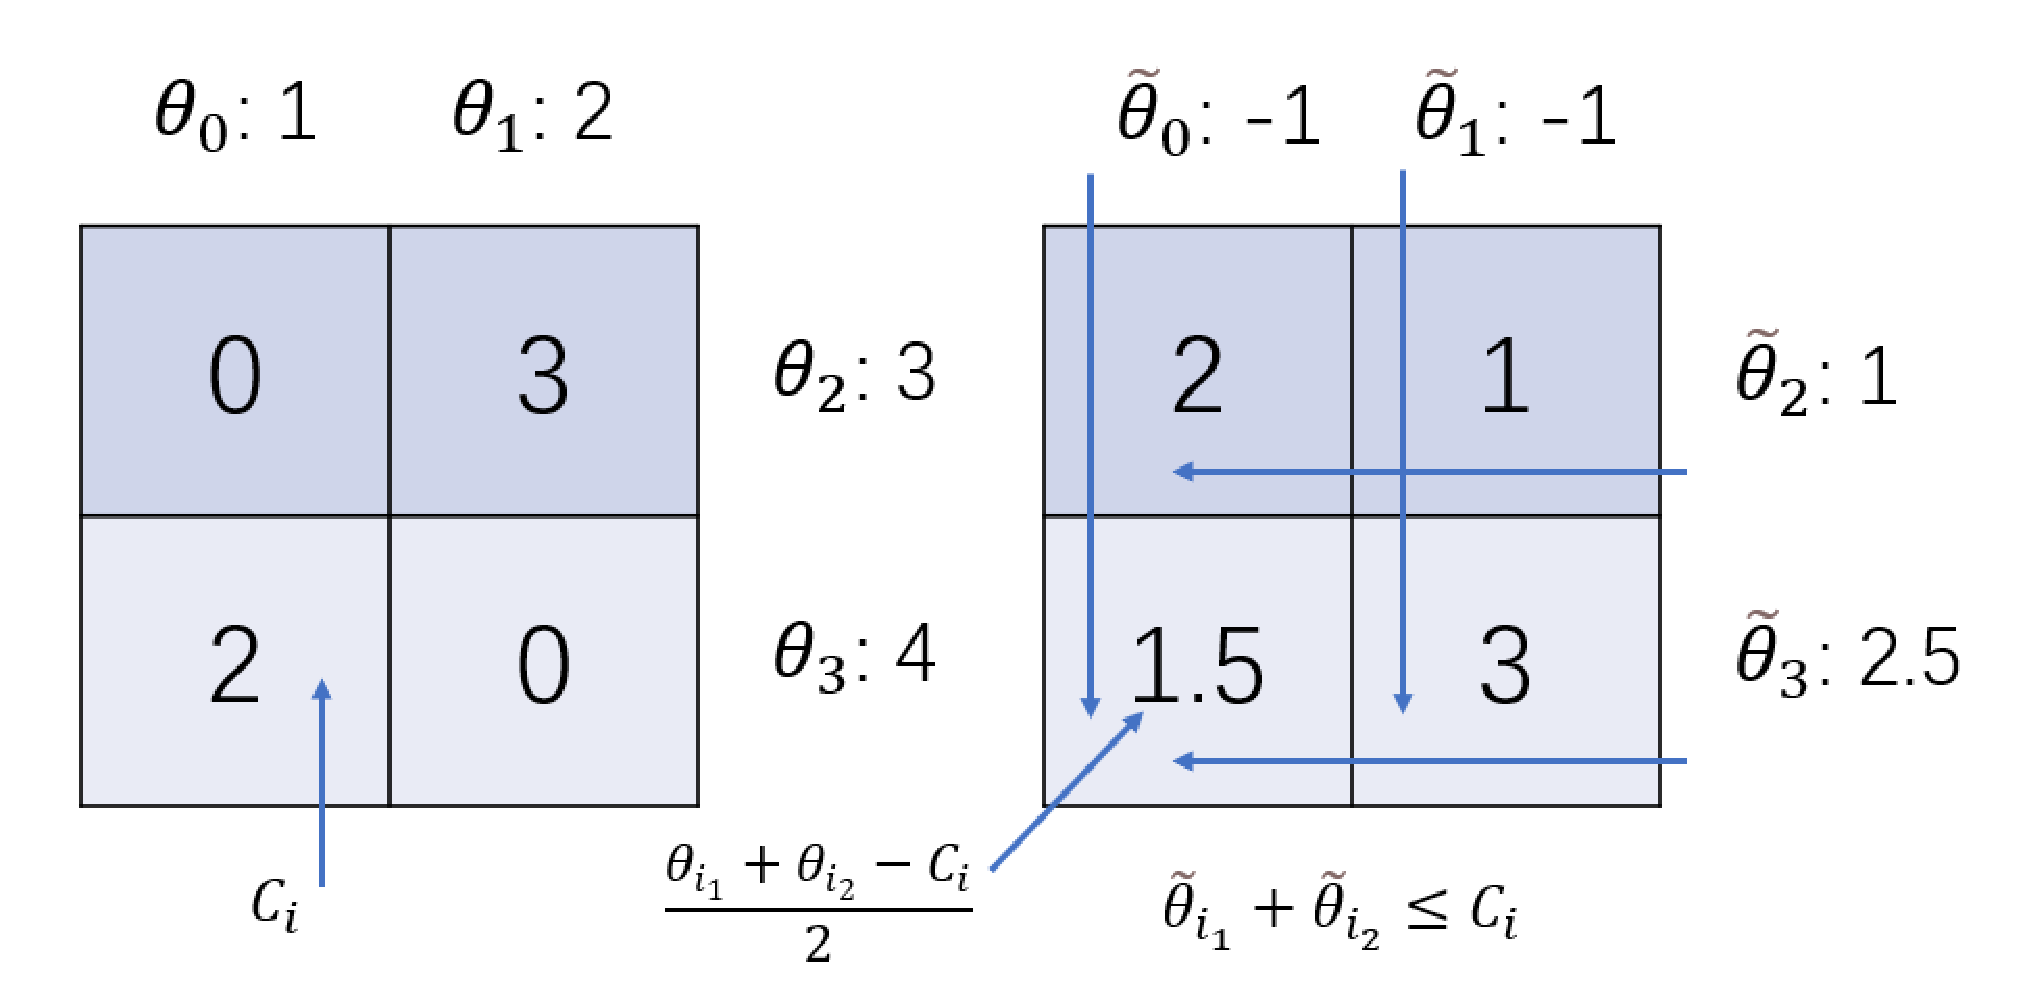
\includegraphics[width = \linewidth]{pic/shifting}
	\caption{Shifting on a 2$\times$2 matrix}
	\end{center}	
	\end{figure}


As we have got the $\tilde{\theta}$ in the $R^{D}$ and we also have another constraint area $\mathcal{R}^{C}$, we are sure that the $\hat{\vt} \in \mathcal{R}^{C}\cap\mathcal{R}^{D}$. However, The intersection of a sphere and a polytope can not be computed in $O(knm)$, where $k$ is a constant. We design a relaxation method. which divides the constraints into two parts, then we maximize the intersection of two hyperplanes and a hyper-ball. 

	\begin{figure}[h]
	\begin{center}	
	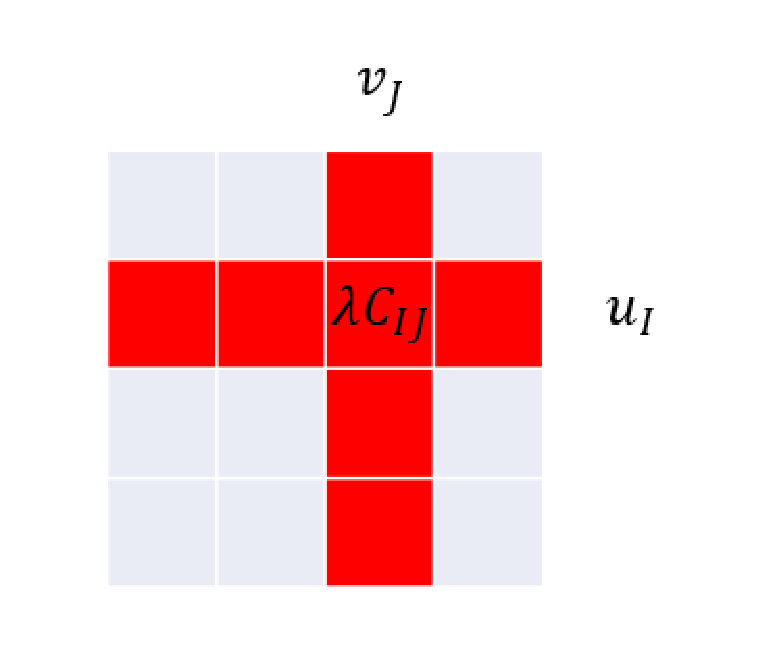
\includegraphics[width = \linewidth]{pic/divide}
	\caption{Selection of group $A_{IJ}$(red) and $B_{IJ}$(grey)}
	\end{center}	
	\end{figure}

\begin{thm}\label{area}(Two plane Screening for UOT) For every single primal variable $t_p$, let $A_p = \{ i \| 0\leq i<nm, i\mid m = I \vee i\mod m = J\}$, $B_p = \{ i \| 0\leq i<nm, i \notin A_p\}$. we can construct the specific area $\mathcal{R}^{S}_{IJ}$ for it.
 \begin{equation}
\begin{split} 
\mathcal{R}^S_{IJ} = \{\theta \|
\begin{aligned}
 &\sum_{l\in A_p}(\theta^{\tranT}\x_{l}\vt_l - \lambda \vc_l \vt)\leq 0 \\
 &\sum_{l\in B_p}(\theta^{\tranT}\x_{l}\vt_l - \lambda \vc_l \vt)\leq 0 \\
  &(\theta-\tilde{\theta})^{\tranT}(\theta-\y)\leq 0
\end{aligned}
\}
\end{split}
\label{eq:divide}
\end{equation}
\end{thm}
We divide the constraints into two groups $A_p$ and $B_p$ for every single $p$, this problem can be solved easily by the Lagrangian method in constant time, the computational process is in Appendix. A


\subsection{Screening Algorithms}

 \begin{algorithm}
 \caption{UOT Dynamic Screening Algorithm}
 \begin{algorithmic}[h]
 \renewcommand{\algorithmicrequire}{\textbf{Input:}}
 \renewcommand{\algorithmicensure}{\textbf{Output:}}
 \REQUIRE $\vt_0, S \in R^{n\times m}, S_{ij}=1, (i,j) = mi+j$
 \ENSURE $S$
 \STATE \text{Choose a solver for the problem.}
 \FOR {$k = 0 \text{ to } K$}
 \STATE $\text{Projection } \tilde{\theta} = \operatorname{Proj}(t^k)$ 
 \FOR {$i = 0 \text{ to } m$}
  \FOR {$j = 0 \text{ to } n$}
  \STATE $\mathcal{R}^{S} \Leftarrow \mathcal{R_{ij}}^S{(\tilde{\theta},t^k)}$
   \STATE $S \Leftarrow {S_{ij} = 0 \text{ if } \max_{\theta \in \mathcal{R}^S} {x_{(i,j)}}^{\tranT}\theta <\lambda c_{(i,j)} }$
 \ENDFOR
  \ENDFOR
 \FOR {$(i,j) \in \{(i,j)\|S_{ij}=0\}$}
  \STATE $\vt^k_{(i,j)} \Leftarrow 0$
  \ENDFOR
  \STATE $\vt^{k+1} = \operatorname{update}(\vt^k)$
 \ENDFOR
  
 \RETURN $\vt^{K+1}, S $ 
 \end{algorithmic} 
 \end{algorithm}

The screening method is irrelevant to the optimization solver you choose. We give the specific algorithm for $L_2$ UOT problem to show the whole optimization process. The $\operatorname{update}$ indicates the updating process for $\vt$ according to the optimizer you choose.\\












































%\section{Experiments}
In this section, we show the efficacy of the proposed methods using a toy Gaussian model and the MNIST dataset.
\subsection{Screening Ratio}
%\section{Conclusion}
Our algorithm is great, we are going to apply the method onto Sinkhorn

\begin{abstract}
\note{HK comment:  We change the story: (OT and UOT $\rightarrow$ Lasso-type UOT $\rightarrow$ Propose Screening (No literature) $\rightarrow$ Evaluation)}
The Safe Screening technique saves computational time by freezing the zero elements in the sparse solution of the Lasso problem. Recently, researchers have linked the UOT problem to the Lasso problem. In this paper, we apply the newest Dynamic Screening framework to the $L_2$ penalized Unbalanced Optimal Transport (UOT) problem. We firstly apply the Screening method onto the UOT problem. We find out that the specific structure for the UOT problem allows it to get better screening results than the Lasso problem. We propose the new Dynamic Screening algorithm and demonstrate its extraordinary effectiveness and potential to benefit from the unique structure of the UOT problem, our algorithm substantially improves the screening efficiency compared to the ordinary Lasso algorithm without significantly increasing on the computational complexity. We demonstrate the advantages of the algorithm through some experiments on the Gaussian distributions and the MNIST dataset.
\end{abstract}


\section{INTRODUCTION}
Optimal Transfer (OT) has a long history in mathematics and has recently become prevalent due to its important role in the machine learning community for measuring distances between histograms. It has outperformed traditional methods in many different areas such as domain adaptation \citep{7586038}, generative models \citep{arjovsky2017wasserstein},, graph machine learning \citep{NEURIPS2019_fdd5b16f} and natural language processing. \citep{084adf2f555549c493e0331a00e4ecad} Its popularity is attributed to the introduction of Sinkhorn's algorithm for the entropy optimal transmission problem, \citep{NIPS2013_af21d0c9} which performs faster in large scale OT problem than the Simplex's method. In order to extend the OT problem, which can only handle balanced samples, to a wider range of unbalanced samples. The unbalanced optimal transport (UOT) is proposed by modifying the restriction term to a penalty function term. UOT has been used in several applications like computational biology \citep{SCHIEBINGER2019928} , machine learning \citep{DBLP:conf/aistats/JanatiCG19} and deep learning \citep{DBLP:conf/iclr/YangU19}. 

The UOT problem is a penalized version of Kantorovich formulation which replaced the equality constraints with penalty functions on the marginal distributions with a divergence. Many different divergences have been taken into consideration for UOT problems like $KL$ divergence, $L_1$ norm, and $L_2$ norm. When it comes to the solving method, $KL$ penalty with the entropy form can be solved by the Sinkhorn algorithm. It provides the UOT computation with scalability and differentiability but suffers from a larger error of $KL$ divergence and lack of sparsity in solution compared with other regularizers \citep{DBLP:conf/aistats/BlondelSR18}. However, $L_2$-norm reguralization could bring a sparse solution, which attracted the attention of researchers and many new algorithms are developed for it \citep{NEURIPS2021_c3c617a9,https://doi.org/10.48550/arxiv.2202.03618} \note{HK comment: As my comments below, the following descriptions should be located below. At the same time, The link between the UOT problem with many other well-known problems such as non-negative matrix decomposition and Lasso problem has been discovered, which encourages researchers to improve it by using the rich results in these fields.}


\note{HK comment: (We mentioned, so far, OT and UTO. Now, we raise a computational problem of OT/UOT). Then, focusing on the Lasso-type reformulation of OT/UOT proposed in the literature, we newly propose a screening technique designated to UOT. But, this extension is NOT trivial because XXXXXX (difference and difficulty). For this we particularly propose a XXXX screening technique for UOT. For this, the detailed explanation  of Screening are not needed. Some paper should be cited, and some basic concept should be provided briefly. ) }


The OT and UOT problems produce extremely sparse solutions due to the effectiveness of their optimal transport cost, which is a similar operator to the Lasso problem. We believe that it indicates the potential effectiveness of applying screening technical in the Lasso problem to the UOT problem. Furthermore, Different from the Lasso problem which has a dense constraints matrix, the UOT problem's constraint matrix is extremely sparse and has a unique transport matrix structure, which would benefit the design of screening and the outcome.


\textbf{Contributions \note{(should be strengthen)}.}: 
\note{
\begin{itemize}
\item We systematically provide the newest framework for the Screening method on the UOT problem. Considering the sparse and specific structure of the UOT problem, we design a new projection method for UOT screening, which hugely improves the screening performance over the general Lasso method.
\item We propose a two-plane screening method for UOT problems, which benefits from UOT's sparse constraints and outperforms the ordinary methods adding only a negligible amount of computation
\end{itemize}
}

\changeHK{The paper is organized as follows. {\bf Section 2} presents preliminary descriptions of optimal transport and unbalanced optimal transport. The screening methods in Lasso-like problems are explained by addressing a dynamic screening framework. In {\bf Section 3}, our proposed screening method for the UOT problem is detailed.  {\bf Section 4} shows numerical experiments. }

\section{PRELIMINARIES}

$\mathbb{R}^n$ denotes $n$-dimensional Euclidean space, and $\mathbb{R}^n_+$ denotes the set of vectors in which all elements are non-negative. $\mathbb{R}^{m \times n}$ represents the set of $m \times n$ matrices. Also, $\mathbb{R}^{m \times n}_+$ stands for the set of $m \times n$ matrices in which all elements are non-negative. We present vectors as bold lower-case letters $\vec{a},\vec{b},\vec{c},\dots$ and matrices as bold-face upper-case letters $\mat{A},\mat{B},\mat{C},\dots$. The $i$-th element of $\vec{a}$ and the element at the $(i,j)$ position of $\mat{A}$ are represented respectively as $\vec{a}_i$ and $\mat{A}_{i,j}$. In addition, $\one_n \in \mathbb{R}^n$ is the $n$-dimensional vector in which all the elements are one. For $\vec{x}$ and $\vec{y}$ of the same size, $\langle \vec{x},\vec{y} \rangle = \vec{x}^T\vec{y}$ is the Euclidean dot-product between vectors. For two matrices of the same size $\mat{A}$ and $\mat{B}$, $\langle \mat{A},\mat{B}\rangle={\rm tr}(\mat{A}^T\mat{B})$ is the Frobenius dot-product. For a vector $\vec{x}$, the $i$-th element of $\exp (\vec{x})$ and $\log (\vec{x})$ respectively represent $\exp (\vec{x}_i)$ and $\log (\vec{x}_i)$. $\mathrm{KL}(\vec{x},\vec{y})$ stands for the KL divergence between $\vec{x} \in \mathbb{R}_+^n$ and $\vec{y} \in \mathbb{R}_+^n$, which is defined as $\sum_i \vec{x}_i \log {(\vec{x}_i/\vec{y}_i)} - \vec{x}_i + \vec{y}_i$. \changeHK{$D_h$ is the Bregman divergence with the strictly convex and differentiable function $h$, i.e., $D_h(\vec{a},\vec{b})=\sum_{i} d_h(a_i, b_i)=\sum_i [h(a_i) - h(b_i) - h'(a_i)(a_i -b_i)]$. In addition, a vectorization operator for $\mat{A} \in \mathbb{R}^{m \times n}$ into $\vec{a} \in \mathbb{R}^{mn}$ is defined as $\vec{a}=\text{vec}(\mat{A})=[\mat{A}_{1,1}, \mat{A}_{1,2}, \cdots, \mat{A}_{m,n-1}, \mat{A}_{m,n}]$, which concatenates the row vectors of a matrix. (check\ it).}
 


\subsection{Optimal Transport and Unbalanced Optimal Transport}
{\bf Optimal Transport (OT):} Given two histograms $\vec{a}\in \R^{m}, \vec{b} \in \R^{n},$ For a cost matrix $\mat{C} \in \mathbbm{R_{+}}^{m \times n}$, mordern Optimal transport problem is trying to get a corresponding transport matrix $\mat{T} \in \R_{+}^{m \times n}$ that minimize the whole transport cost, which could be formulated as:
\begin{eqnarray}
\label{Eq:Standard_OT}
\operatorname{OT}(\vec{a},\vec{b}) &:=& \min_{ \mat{T} \in \R_{+}^{m \times n}} \langle \mat{C}, \mat{T} \rangle \\
\text{subject\ to}&& \mat{T} \one_n= \vec{a}, \mat{T}^{T}\one_m = \vec{b}. \notag
\end{eqnarray}

Defining $\vec{t} = \text{vec}({\mat{T}}) \in \mathbbm{R}^{mn}$ and $\vec{c} = \text{vec}({\mat{C}}) \in \mathbbm{R}^{mn}$, we reformulate Eq.(\ref{Eq:Standard_OT}) in a vector format as
\begin{eqnarray}
\label{Eq:Vector_OT}
\operatorname{OT}(\vec{a},\vec{b}) &:=& \min_{\vec{t} \in \R_{+}^{\changeHK{mn}}} \vec{c}^{\tranT}\vec{t} \\
\text{subject\ to}&& \mat{N}\vec{t} = \vec{a}, \mat{M}\vec{t} = \vec{b}, \notag
\end{eqnarray}
\changeHK{where $\mat{N} \in \R^{m \times mn}$ and $\mat{M} \in \R^{n \times mn}$ are two matrices composed of ``0" and ``1". $\mat{N}$ and $\mat{M}$ in case of $m=n=3$ are given, respectively, as}
\begin{equation*}
\begin{split}
\mat{N}&=\begin{pmatrix}
1&1&1& 0& 0& 0& 0& 0&0\\
0 & 0& 0&1&1&1& 0& 0&0\\
0 & 0& 0& 0& 0& 0&1&1&1\\
\end{pmatrix},\\
\mat{M}&=\begin{pmatrix}
 1& 0& 0&1& 0& 0&1& 0&0\\
 0&1& 0& 0&1& 0& 0&1&0\\
 0& 0&1& 0& 0&1& 0& 0&1\\
 \end{pmatrix}.
  \end{split}
 \end{equation*}
 
{\bf Unbalanced Optimal Transport (UOT):} The UOT problem is a penalized version of Kantorovich formulation which replaced the equality constraints with penalty functions on the marginal distributions with a divergence. 
Although $\|\vec{a}\|_2 = \|\vec{b}\|_2$ holds in the OT problem, the solution $\hat{\vec{t}}$ does not exist when $\|\vec{a}\|_2 \neq \|\vec{b}\|_2$. However, allowing $\|\vec{a}\|_2 \neq \|\vec{b}\|_2$, we derive the UOT problem as follows. Defining $\vec{y} = [\vec{a}, \vec{b}]^{\tranT}$ and $\mat{X} = [\mat{M}^{\tranT},\mat{N}^{\tranT}]^{\tranT}$, the UOT problem can be defined introducing a penalty function for the histograms: 
\begin{equation}
\label{eq:uot}
\operatorname{UOT}(\vec{a},\vec{b}) := \min_{\vec{t} \in \R_{+}^{mn}} \vec{c}^{\tranT}\vec{t} + D_h(\mat{X}\vec{t},\vec{y}),
\end{equation}
where $D_h$ is the Bregman divergence. 

{\bf Relationship with Lasso:} 
The lasso-like problem has a general formula:
%
\begin{eqnarray}
f(\vec{t}) &:=& g(\vec{t}) + D_h(\mat{X} \vec{t},\vec{y}).
%, t\in \mathbbm{R}^{mn}.
\end{eqnarray}

When $g(\vec{t}) = \lambda \|\vec{t}\|_1$ with $\lambda > 0$ and $D_h(\mat{X} \vec{t},\vec{y}) = \|\mat{X} \vec{t}-\vec{y}\|_2^2$, this problem is reduced to the $L_2$-regunarlized regression Lasso problem. It should be noted that $\mat{X}$ in UOT is different from the one in the Lasso problem. More concretely, the former $\mat{X}$ has a specific structure and has only two non-zero elements and is equal to $1$ whereas the latter $\mat{X}$ in Lasso problem is irregular and dense.


\subsection{Dynamic Screening Framework}

\note{Screening is a well-known technique proposed by \citep{ghaoui2010safe} in the field of lasso problems, where the $L_1$ regularizer leads to a sparse solution for the problem. It can pre-select solutions that must be zero theoretically and freeze them before computation. The solutions to many large-scale optimization problems are sparse, and a large amount of computation is wasted on updating the zero elements. With the Safe Screening method, we can identify and freeze the elements that are zero with linear complexity computation before starting the algorithm, thus saving optimization time. the Screening method get attention in recent years and has been improved a lot, New methods such as Dynamic Screening \citep{7128732}, Gap screening method \citep{JMLR:v18:16-577} and Dynamic Sasvi \citep{NEURIPS2021_7b5b23f4}.}

Hereinafter, we briefly detail the framework proposed in \citep{NEURIPS2021_7b5b23f4} to introduce the whole dynamic screening technique for the Lasso-like problem:
\begin{equation}
\label{eq:lassolike}
\min_{\vec{t}} \left\{ f(\vec{t}) := g(\vec{t}) + d(\mat{X} \vec{t}) \right\}.
\end{equation}

The Fenchel-Rockafellar Duality yields the dual problem as presented below:
\begin{thm}[Fenchel-Rockafellar Duality] 
\label{Thm:FRD}
If $d$ and $g$ are proper convex functions on $\mathbbm{R}^{m+n}$ and $\mathbbm{R}^{mn}$. Then we have the following:
 $$
\begin{aligned}
\min_{\vec{t}} g(\vec{t}) + d(\mat{X}\vec{t}) = \max_{\vec{\vec{\theta}}} -d^*(-\vec{\theta})-g^*(\mat{X}^{\tranT}\vec{\theta})
\end{aligned}
$$
\end{thm}

Because the primal function $d$ is always convex, the dual function $d^*$ is concave. Assuming $d^*$ is an $L$-strongly concave problem, we can design an area for any feasible $\tilde{\vec{\theta}}$ by the strongly concave property:

\begin{thm}[$L$-strongly concave \changeHK{\citep[Theorem 5]{NEURIPS2021_7b5b23f4}}]\label{circle}
Considering problem in Eq.(\ref{eq:lassolike}), if function $d$ and $g$ are both convex, for $\forall \ \tilde{\vec{\theta}} \in{R^{m+n}}$ and satisfied the constraints on the dual problem, we have the following area constructed by its L-strongly concave property:  
$$
\begin{aligned}
\mathcal{R}^{C}:=\vec{\theta} \in \left\{\frac{L}{2}\|\vec{\theta}-\tilde{\vec{\theta}}\|_2^2+d^*(-\tilde{\vec{\theta}}) \leq d^*(-\vec{\theta})\right\}.
\end{aligned}
$$
\end{thm}

We know that the optimal solution for the dual problem $\hat{\vec{\theta}}$ satisfied the inequality, so the set is not empty.



\section{PROPOSED UOT SCREENING}

\changeHK{This section proposes a dynamic screening method designated for the UOT problem. For this purpose, we first derive the dual formulation of the Lasso-like formulated UOT problem in Eq.(\ref{eq:uot}). Concrete proofs of lemma and theorems are provided in the supplementary file.}


\subsection{Dual formulation of UOT}

We can get the dual form of the UOT problem: 
For $d(\mat{X} \vec{t}) = \frac{1}{2}\|\mat{X} \vec{t}-\vec{y}\|_2^2$, the dual Lasso problem gives $d^*(-\vec{\theta})$ as
 \begin{equation}
\begin{split} 
d^*(-\vec{\theta}) = \frac{1}{2}\|\vec{\theta}\|_2^2-{\vec{y}^T\vec{\theta}},
 \end{split}
\end{equation}
and  $g^*(\mat{X}^{\tranT}\vec{\theta})$ is given as
 \begin{equation*}
\begin{split} 
g^*(\mat{X}^{\tranT}\vec{\theta}) = 
%\left\{
%\begin{aligned}
%0 \quad&\quad ( \forall \vec{t} \quad\vec{\theta}^{\tranT}\mat{X}\vec{t} - g(\vec{t}) \leq 0 )\\
%\infty \quad&( \exists t \quad\vec{\theta}^{\tranT}\mat{X}\vec{t} - g(\vec{t}) \leq 0 ).
%\end{aligned}
\begin{cases}
0 & (\forall \vec{t} \quad\vec{\theta}^{\tranT}\mat{X}\vec{t} - g(\vec{t}) \leq 0 )\\
\infty &( \exists t \quad\vec{\theta}^{\tranT}\mat{X}\vec{t} - g(\vec{t}) \changeHK{>} 0 ).
\end{cases}
%\right.
 \end{split}
\end{equation*}

For UOT problem in Eq.(\ref{eq:uot}), we obtain its dual form from {\bf Theorem \ref{Thm:FRD}} as
\begin{lem}[Dual form of UOT problem]
For UOT problem in Eq.(\ref{eq:uot}), we have the following dual form:
\begin{equation}
\begin{split}
-d^*(-\vec{\theta}) - g^*(\mat{X}^{\tranT}\vec{\theta})& = -\frac{1}{2}\|\vec{\theta}\|_2^2-\vec{y}^{\tranT}\vec{\theta} \\
 \text{s.t.} \quad \quad \vec{x}_p^{\tranT}\vec{\theta} -\lambda \vec{c}_p &\leq 0, \forall p,
 \end{split}
 \label{eq:uotdual}
\end{equation}
where $\vec{x}_p $ corresponds to the $p$-th column of $\mat{X}$. 
\end{lem}
It is clear that the strongly concave coefficient $L$ for the dual function $d$ is 1. These in-equations in Eq.(\ref{eq:uotdual}) make up a dual feasible area written as $\mathcal{R}^{D}$, and the optimal solution satisfied them.\\
From the KKT condition, we know that for the optimal primal solution $\hat{\vec{t}}$:
\begin{thm}[KKT condition] For the dual optimal solution $\hat{\vec{\theta}}$, we have the following relationship:
 \begin{equation}
\begin{split}
\vec{x}_p^{\tranT}\hat{\vec{\theta}} -\lambda \vec{c}_p \left\{
\begin{aligned}
< 0 \quad& \Rightarrow \hat{\vec{t}}_p = 0\\
= 0 \quad& \Rightarrow \hat{\vec{t}}_p \geq 0.
\end{aligned}
\right.
 \end{split}
 \label{eq:kkt}
\end{equation}
\end{thm}

\subsection{Detailed Screening Method}

Eq.(\ref{eq:kkt}) indicates a potential method to screening the primal variable. Since we do not know the information of $\hat{\vec{t}}$ directly, we construct an area $\mathcal{R}^{S}$ containing the $\hat{\vec{t}}$, if
\begin{equation}
\max_{\vec{t} \in \mathcal{R}^S} \vec{x}_p^{\tranT}\vec{\theta} -\lambda \vec{c}_p < 0.
\end{equation}
Then we have
 \begin{equation}
 \vec{x}_p^{\tranT}\hat{\vec{\theta}} -\lambda \vec{c}_p < 0,
 \label{eq:kktineq}
\end{equation}
which means the corresponding $\hat{\vec{t}}_p = 0$, and can be screened out. Noteworthy point is that, for the UOT problem, $\vec{x}_p = [...,0,1,0,...,0,1,0,...,]^{\tranT}$ has only two nonzero elements, $p_1$ and $p_2$, that are equal to 1. Therefore, we can set $\vec{\theta} = [\vec{u}^{\tranT},\vec{v}^{\tranT}]^{\tranT}$ and $\vec{u}\in\R^{m}, \vec{v}\in\R^{n}$, assuming $p=(I,J)$ where $I = p \mid m, J = p \mod m$. Subsequently, we rewrite Eq.(\ref{eq:kktineq}) as 
%
 \begin{equation}
\vec{u}_{I} + \vec{v}_{J}-\lambda \vec{c}_p < 0.
\end{equation}

Before we start to construct the area containing $\hat{\vec{\theta}}$ from {\bf Theorem \ref{circle}}, we first need to find $\tilde{\vec{\theta}}$ in the dual feasible area $\mathcal{R}^{D}$. Although there exists a relationship between the primal variable and dual variable $\vec{\theta} = \vec{y} - \mat{X}\vec{t}$, we sometimes get $\vec{\theta} \notin \mathcal{R}^{D}$. This requires us to project $\vec{\theta}$ onto $\mathcal{R}^{D}$. In the Lasso problem, as the constraints limit the $\|\vec{x}_p \vec{\theta}\|_1$, and every element of $\vec{\theta}$ is multiplied by a dense $x_i$, one has to use a shrinking method to obtain a $\tilde{\vec{\theta}} \in \mathcal{R}^{D}$ for further constructing the dual screening area \changeHK{\cite{xxxxx}}: 
\begin{equation*}
\tilde{\vec{\theta}} = \frac{\lambda \vec{c} ^{\tranT}(\vec{y} - \mat{X} \vec{t})}{\max(\lambda \vec{c}, \|\mat{X}^{\tranT}(\vec{y}-\mat{X}\vec{t})\|_{\infty})}
\end{equation*}

%Unlike in the Lasso problem, 
This projection pushes the $\vec{\theta}$ far away from the optimum $\hat{\vec{\theta}}$, and cannot work well when one of the costs is $\vec{c}_p = 0$. This situation fortunately never happens in the Lasso problem \changeHK{because xxxx}, however, frequently happens in the UOT problem. Under this situation, the whole dual elements would degenerate to zero and disable the screening process. Therefore, noting that, fo the UOT problem, it only allows $\vec{t}_p \geq 0$, and the $\vec{x}_p$ only consists of two non-zero elements, we can adapt a better projection method. The following theorem states this:
\begin{thm}[UOT shifting projection]
\label{Thm:UOT_ShiftProjection}
For any $\vec{\theta} = [{\vec{u}}^{\tranT},{\vec{v}}^{\tranT}]^{\tranT}$, we compute the projection $\tilde{\vec{\theta}} = [\tilde{\vec{u}}^{\tranT},\tilde{\vec{v}}^{\tranT}]^{\tranT} \in \mathcal{R}^{D}$ as
\begin{eqnarray}
\tilde{\vec{u}}_I &=& {\vec{u}}_I - \max_{0\changeHK{\leq} j\changeHK{\leq} n} \frac{{\vec{u}}_I +{\vec{v}}_j - \lambda\vec{c}_{p}}{2} \notag\\
& =& \frac{{\vec{u}}_I +\lambda\vec{c}_{p}}{2} - \frac{1}{2}\max_{0\changeHK{\leq} j\changeHK{\leq} n} {\vec{v}}_j\\
\tilde{\vec{v}}_J &=& {\vec{v}}_J - \max_{0 \changeHK{\leq} i \changeHK{\leq} m} \frac{{\vec{u}}_i +{\vec{v}}_J - \lambda\vec{c}_{p}}{2}\notag\\
& =& \frac{{\vec{v}}_J +\lambda\vec{c}_{p}}{2} - \frac{1}{2}\max_{0\changeHK{\leq} i\changeHK{\leq} m} {\vec{u}}_j
 \label{eq:uotproj}
\end{eqnarray}
\end{thm}
	\begin{figure}[h]
	\begin{center}	
	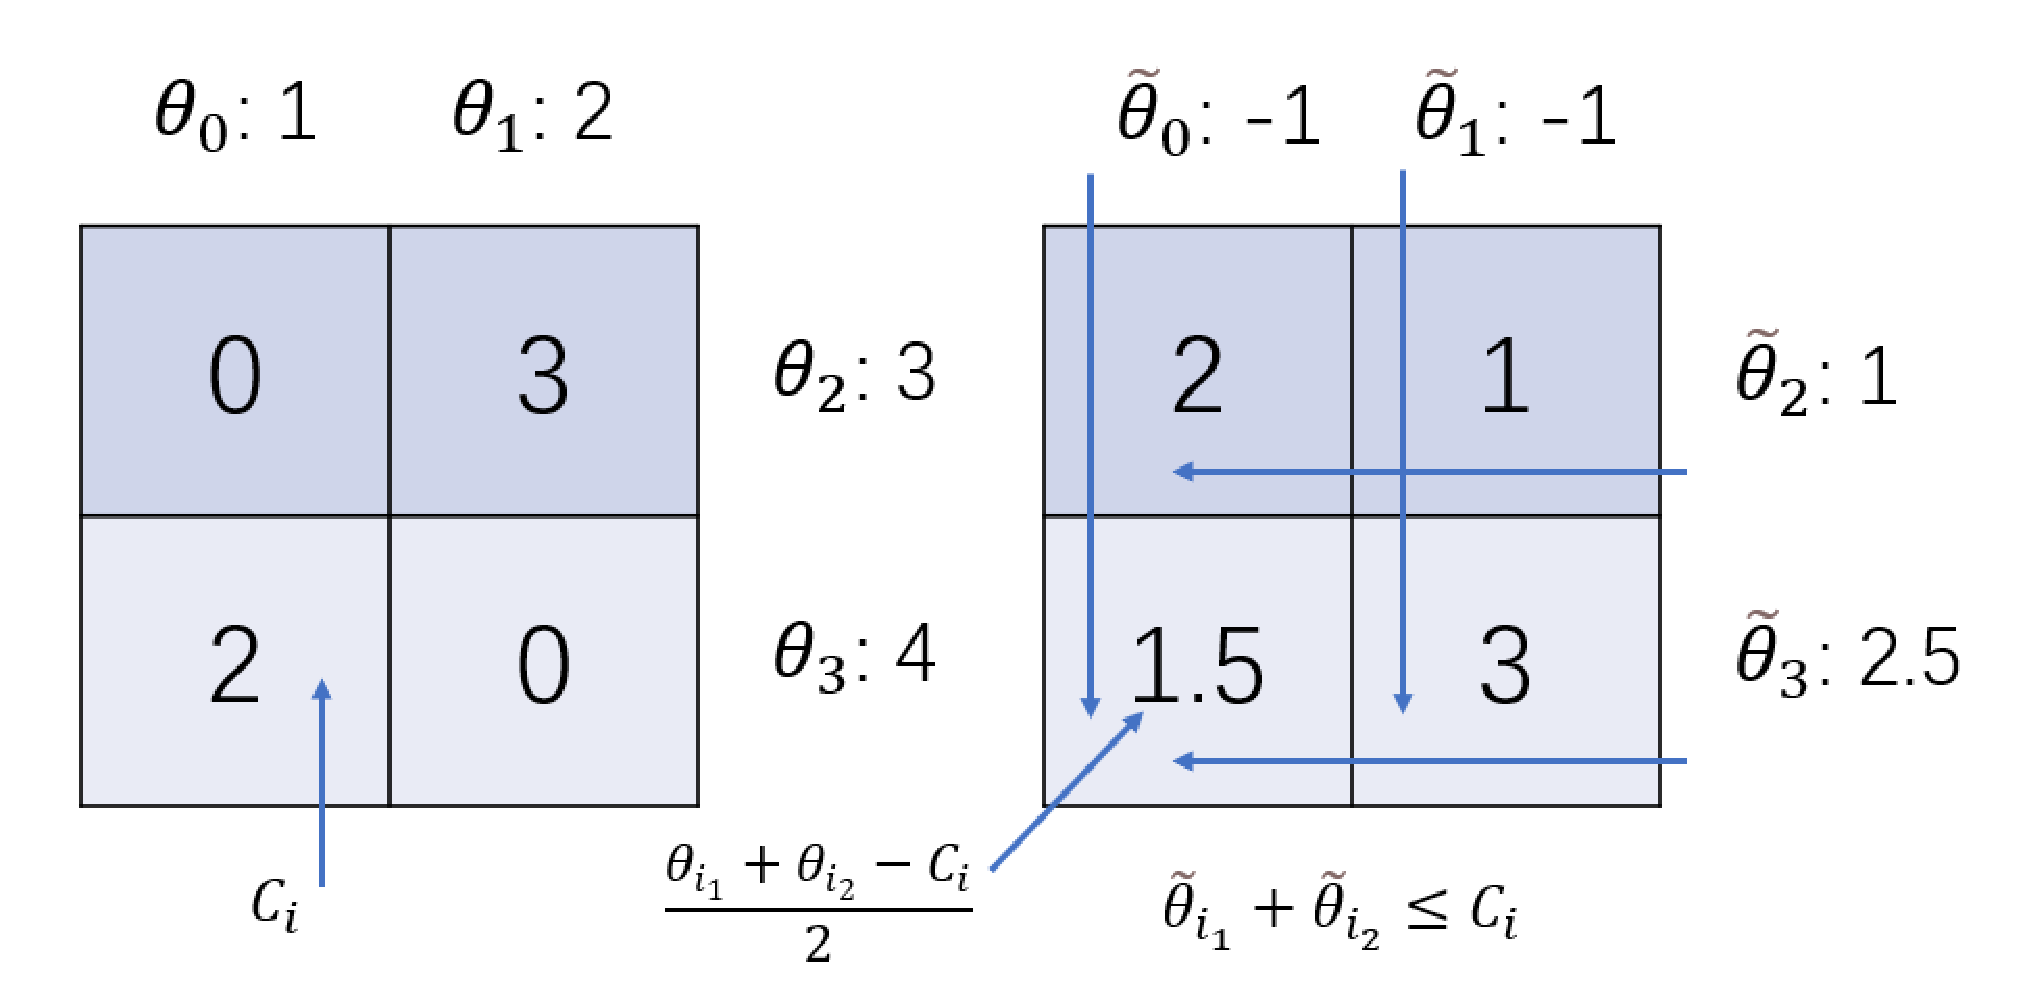
\includegraphics[width = \linewidth]{pic/shifting}
	\caption{Shifting on a 2$\times$2 matrix}
	\end{center}	
	\end{figure}


Since we now obtain $\tilde{\vec{\theta}}$ in $\mathcal{R}^{D}$, we additionally consider $\mathcal{R}^{C}$ in {\bf Theorem \ref{circle}} to satisfy $\hat{\vec{t}} \in \mathcal{R}^{C}\cap\mathcal{R}^{D}$. However, the intersection of a sphere and a polytope cannot be computed \note{(????)} in $O(knm)$, where $k$ is a constant. Therefore, we propose a relaxation method, denoted as {\it two plane screening}. This divides the constraints into two parts, then we maximize the intersection of two hyperplanes and a hyper-ball. The next theorem states this:
%
\begin{thm}[Two plane screening for UOT]
\label{Thm:AreaScreeningUOT}
For every single primal variable $t_p$, let $A_p = \{ i \| 0\leq i<nm, i\mid m = I \vee i\mod m = J\}$, $B_p = \{ i \| 0\leq i<nm, i \notin A_p\}$. Then, we construct a specific area $\mathcal{R}^{S}_{IJ}$ as presented below:
 \begin{equation}
\begin{split} 
\mathcal{R}^S_{IJ} = \left\{\vec{\theta} \ \left|\!\left| \ 
\begin{aligned}
 &\sum_{l\in A_p}(\vec{\theta}^{\tranT}\vec{x}_{l}\vec{t}_l - \lambda \vec{c}_l \vec{t})\leq 0, \\
 &\sum_{l\in B_p}(\vec{\theta}^{\tranT}\vec{x}_{l}\vec{t}_l - \lambda \vec{c}_l \vec{t})\leq 0, \\
  &(\vec{\theta}-\tilde{\vec{\theta}})^{\tranT}(\vec{\theta}-\vec{y})\leq 0 \ (\note{\text{where from??}})
\end{aligned}
\right.\right.
\right\}.
\end{split}
\label{eq:divide}
\end{equation}
\end{thm}

\note{How does $\mathcal{R}^{S}_{IJ}$ play in the following??? Is in Algorithm 1 only?}



We divide the constraints into two groups $A_p$ and $B_p$ for every single $p$, this problem can be solved easily by the Lagrangian method in constant time, the computational process is in Appendix. A

	\begin{figure}[h]
	\begin{center}	
	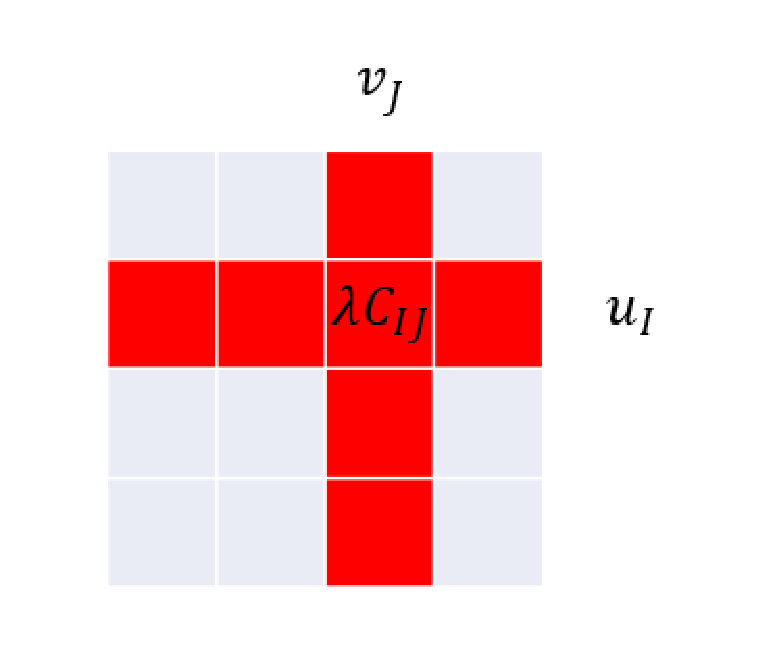
\includegraphics[width = 0.7\linewidth]{pic/divide}
	\caption{Selection of group $A_{IJ}$(red) and $B_{IJ}$(grey)}
	\end{center}	
	\end{figure}

\subsection{Screening Algorithms}

 \begin{algorithm}
 \caption{UOT Dynamic Screening Algorithm}
 \begin{algorithmic}[h]
 \label{Alg:UOTDynamicScreening}
 \renewcommand{\algorithmicrequire}{\textbf{Input:}}
 \renewcommand{\algorithmicensure}{\textbf{Output:}}
 \REQUIRE $\vec{t}_0, S \in R^{n\times m}, S_{ij}=1, (i,j) = mi+j$
 \ENSURE $S$
 \STATE \text{Choose a solver for the problem.}
 \FOR {$k = 0 \text{ to } K$}
 \STATE $\text{Projection } \tilde{\vec{\theta}} = \operatorname{Proj}(\vec{t}^k)$ 
 \FOR {$i = 0 \text{ to } m$}
  \FOR {$j = 0 \text{ to } n$}
  \STATE $\mathcal{R}^{S} \leftarrow \mathcal{R}_{ij}^S{(\tilde{\vec{\theta}},\vec{t}^k)}$
   \STATE $S \leftarrow {S_{ij} = 0 \text{ if } \max_{\vec{\theta} \in \mathcal{R}^S} {x_{(i,j)}}^{\tranT}\vec{\theta} <\lambda c_{(i,j)} }$
 \ENDFOR
  \ENDFOR
 \FOR {$(i,j) \in \{(i,j)\|S_{ij}=0\}$}
  \STATE $\vec{t}^k_{(i,j)} \leftarrow 0$
  \ENDFOR
  \STATE $\vec{t}^{k+1} = \operatorname{update}(\vec{t}^k)$
 \ENDFOR
   \RETURN $\vec{t}^{K+1}, S $ 
 \end{algorithmic} 
 \end{algorithm}
 \note{(Insert equation numbers in appropriate lines in {\bf Algorithm \ref{Alg:UOTDynamicScreening)}}}

It should be emphasized that the proposed screening method is {\it independent} of the optimization solver that you choose. We give the specific algorithm for $L_2$ UOT problem to show the whole optimization process as in {\bf Algorithm \ref{Alg:UOTDynamicScreening}}. The $\operatorname{update}(\vec{t})$ operator in the algorithm indicates the updating process for $\vec{t}$ according to the adopted optimizer.\\

\subsection{Computational Cost Analysis}

\note{XXXXXX}

\section{EXPERIMENTS}
In this section, we show the efficacy of the proposed methods using toy Gaussian models and the MNIST dataset.
\subsection{Projection Method}
To prove the effectiveness of our projection method compared with the traditional projection method in the Lasso problem, we compared the projection distance and screening ratio with randomly generated Gaussian measures by two projection methods. We set the $\lambda = \frac{\|\mathbf{X}^{\tranT}y\|}{100}$ and test for 10 different pairs.We choose the FISTA for solving the $L_2$ penalized UOT problems. Our projection method has only moved the dual point by a very small order of magnitude. It ensures that the points are kept at a smaller distance from the optimal solution and cause better screening effects.
	\begin{figure}[h]
	\begin{center}	
	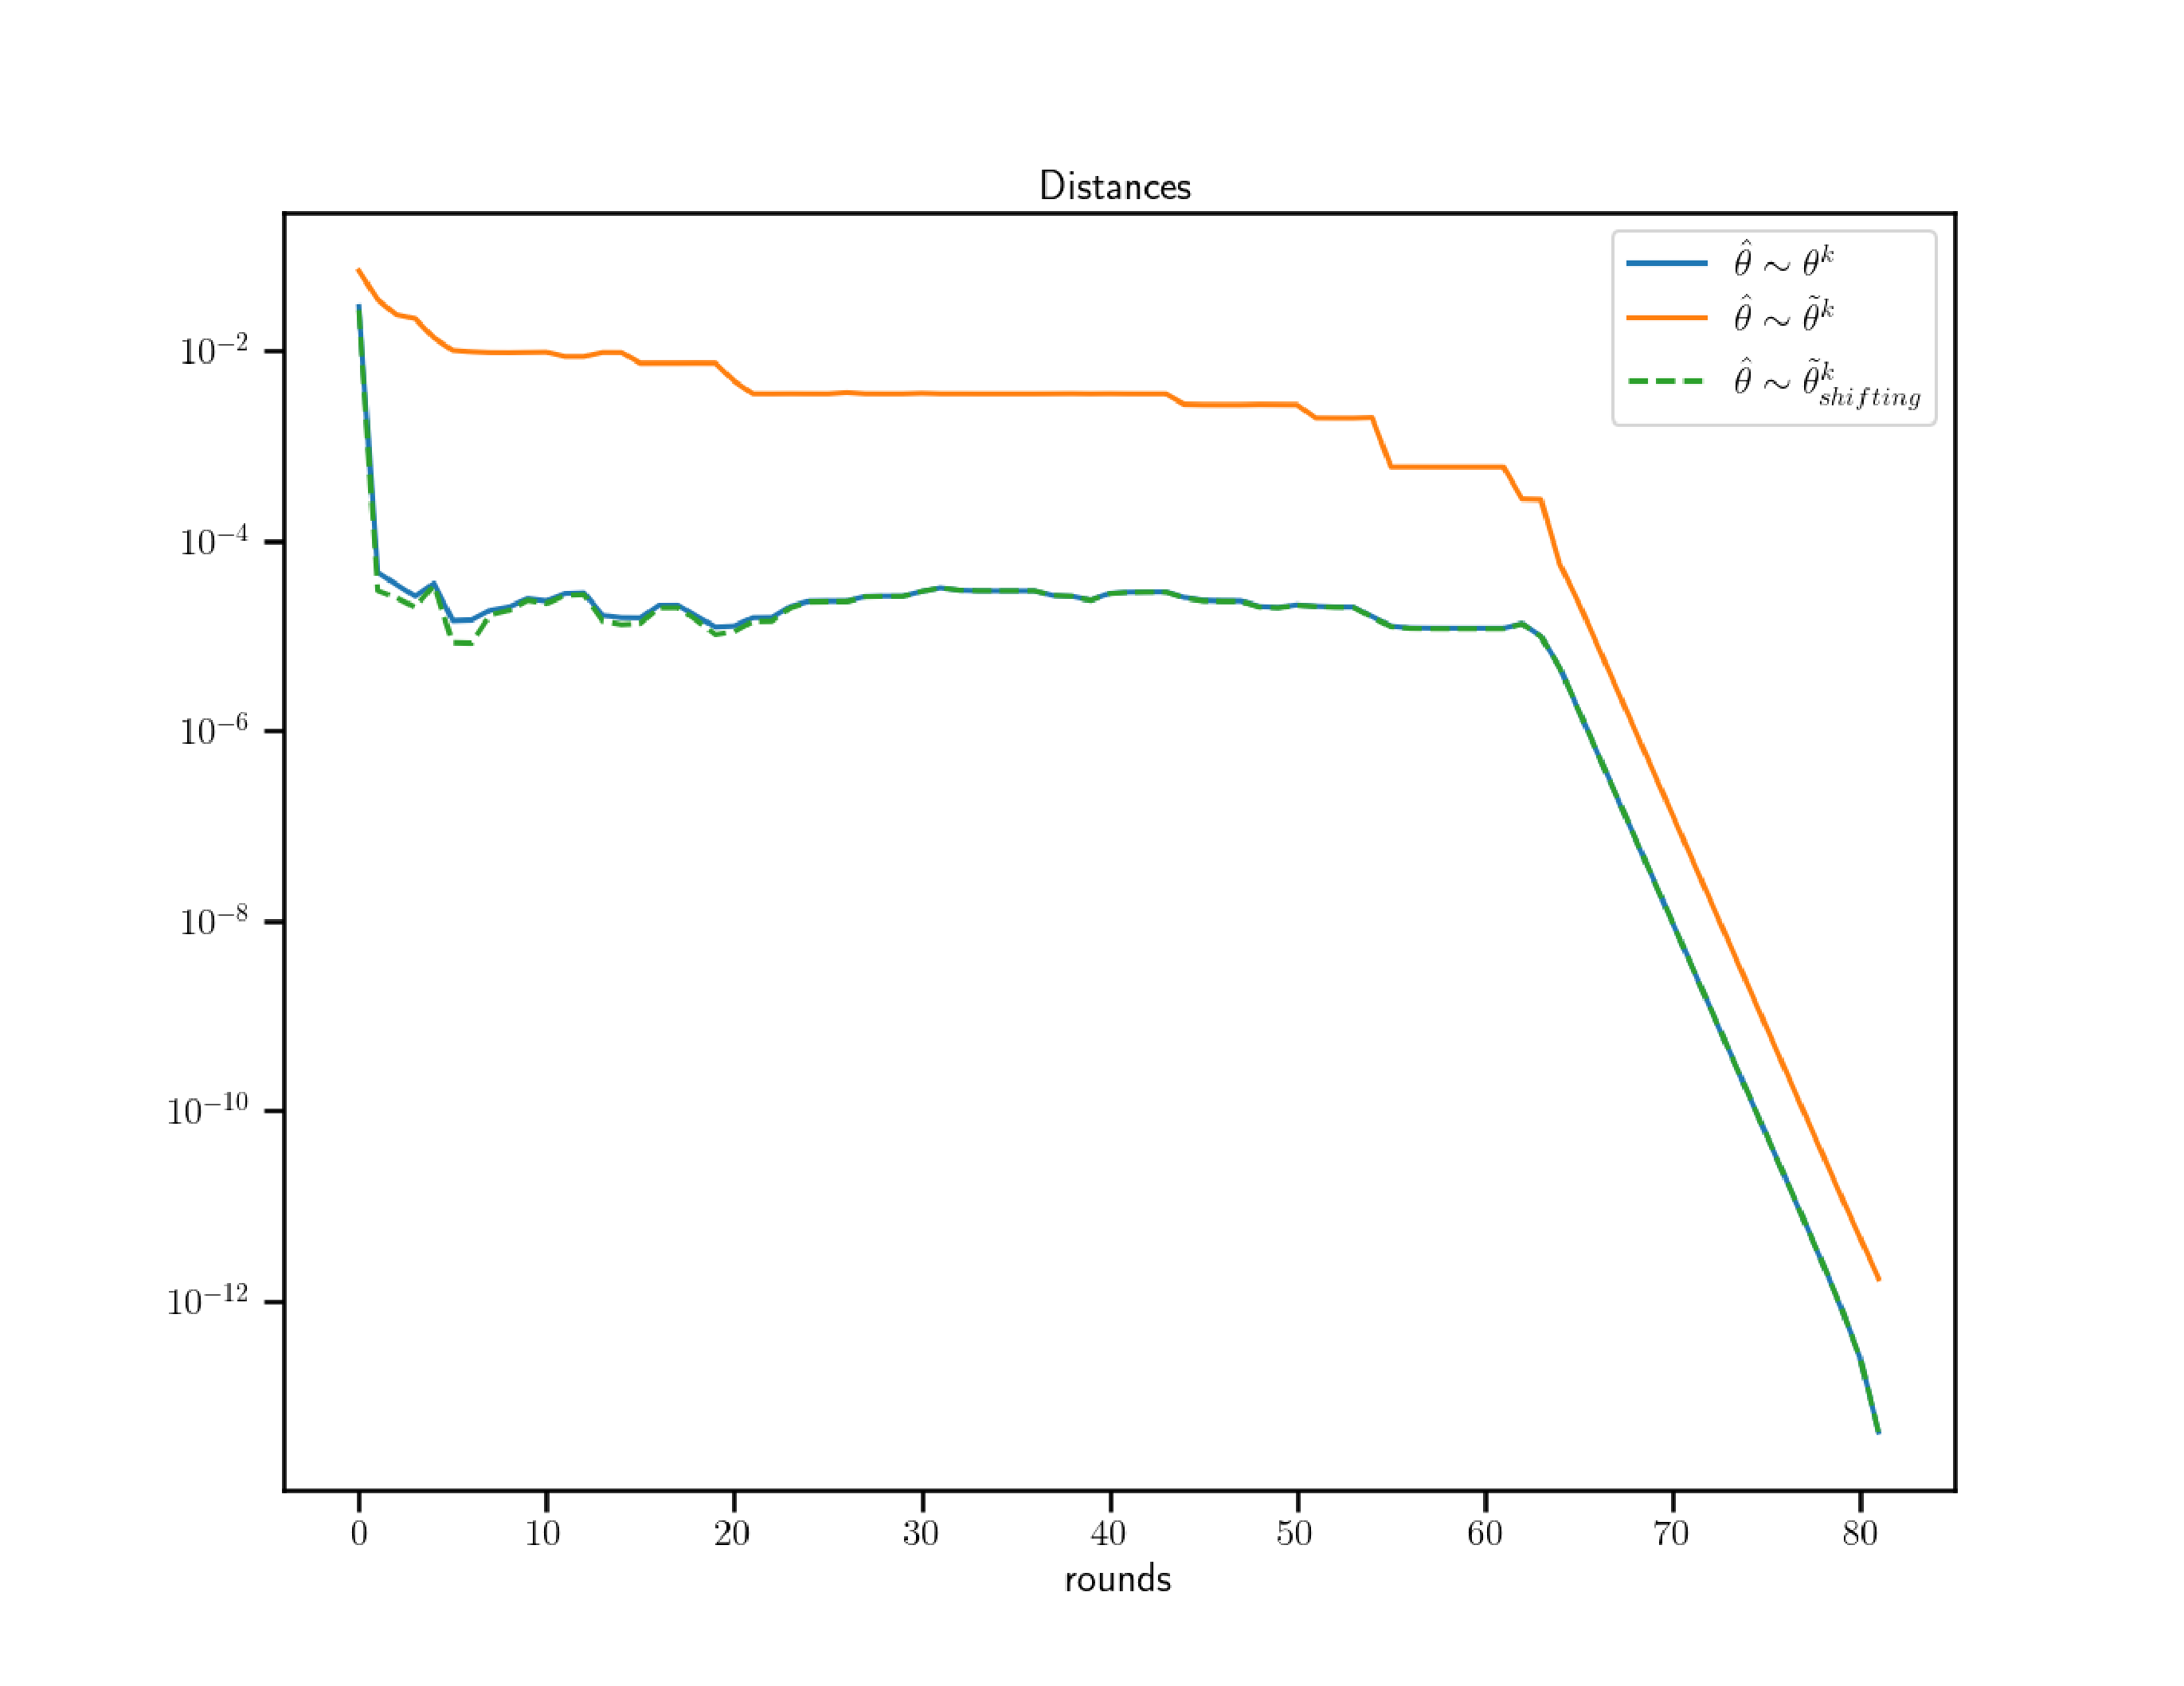
\includegraphics[width = \linewidth]{pic/projdis}
	\caption{Distance of different projection method}
	\end{center}	
	\end{figure}
	\begin{figure}[htbp]
	\begin{center}	
	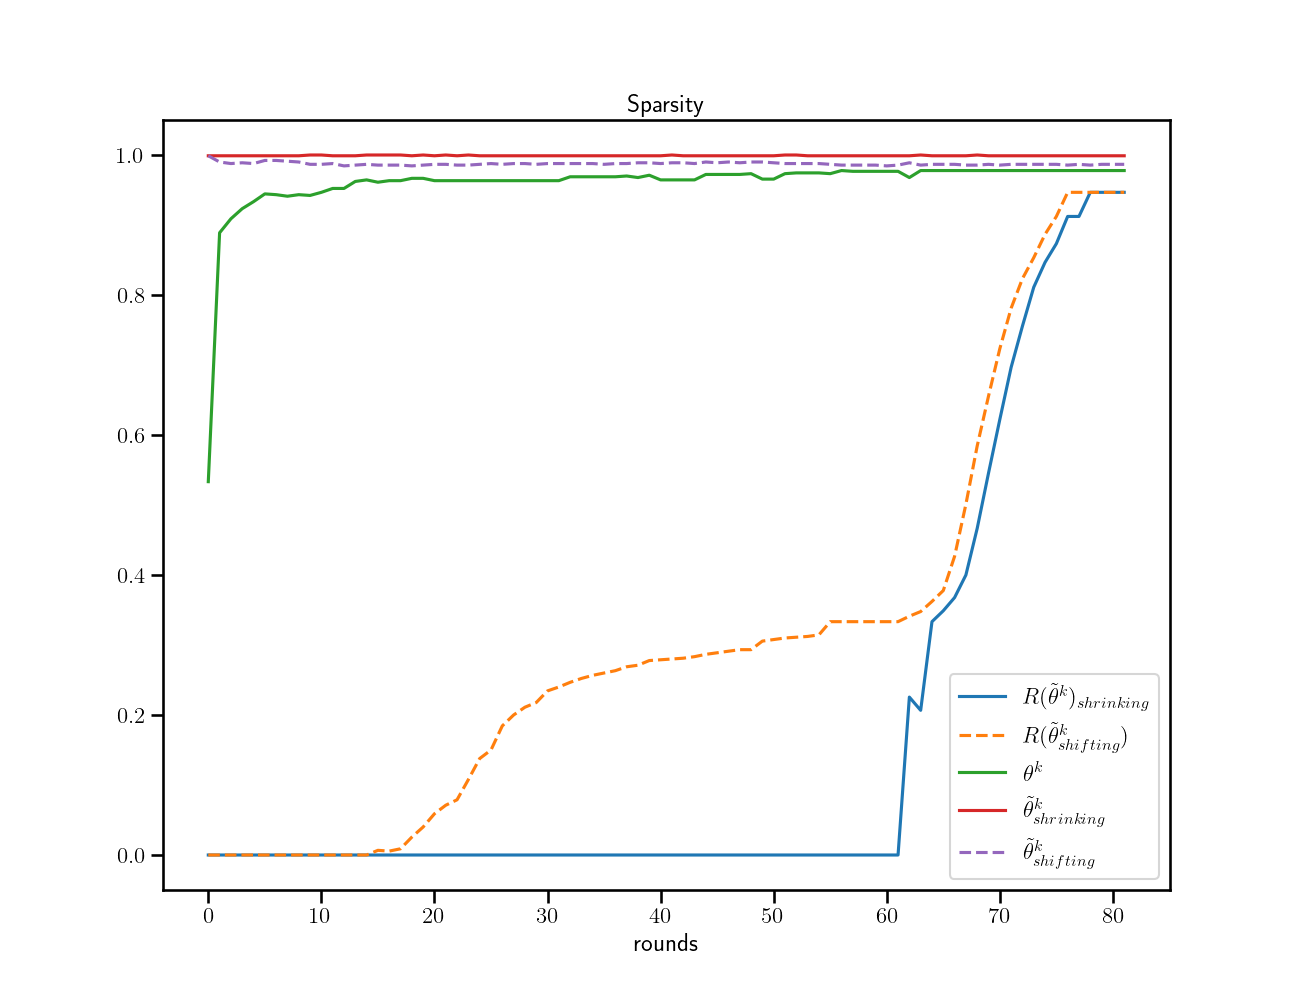
\includegraphics[width = \linewidth]{pic/sparse_proj}
	\caption{Screening ratio of different projection method}
	\end{center}	
	\end{figure}

\subsection{Divide Method}
We compared the screening ratio with three different methods, including our Divide method, Dynamic Sasvi method, and Gap method. Every method would use our projection method to get a better outcome, which also makes sure the difference in performance is only in the construction of the feasible domain. 
	\begin{figure}[h]
	\begin{center}	
	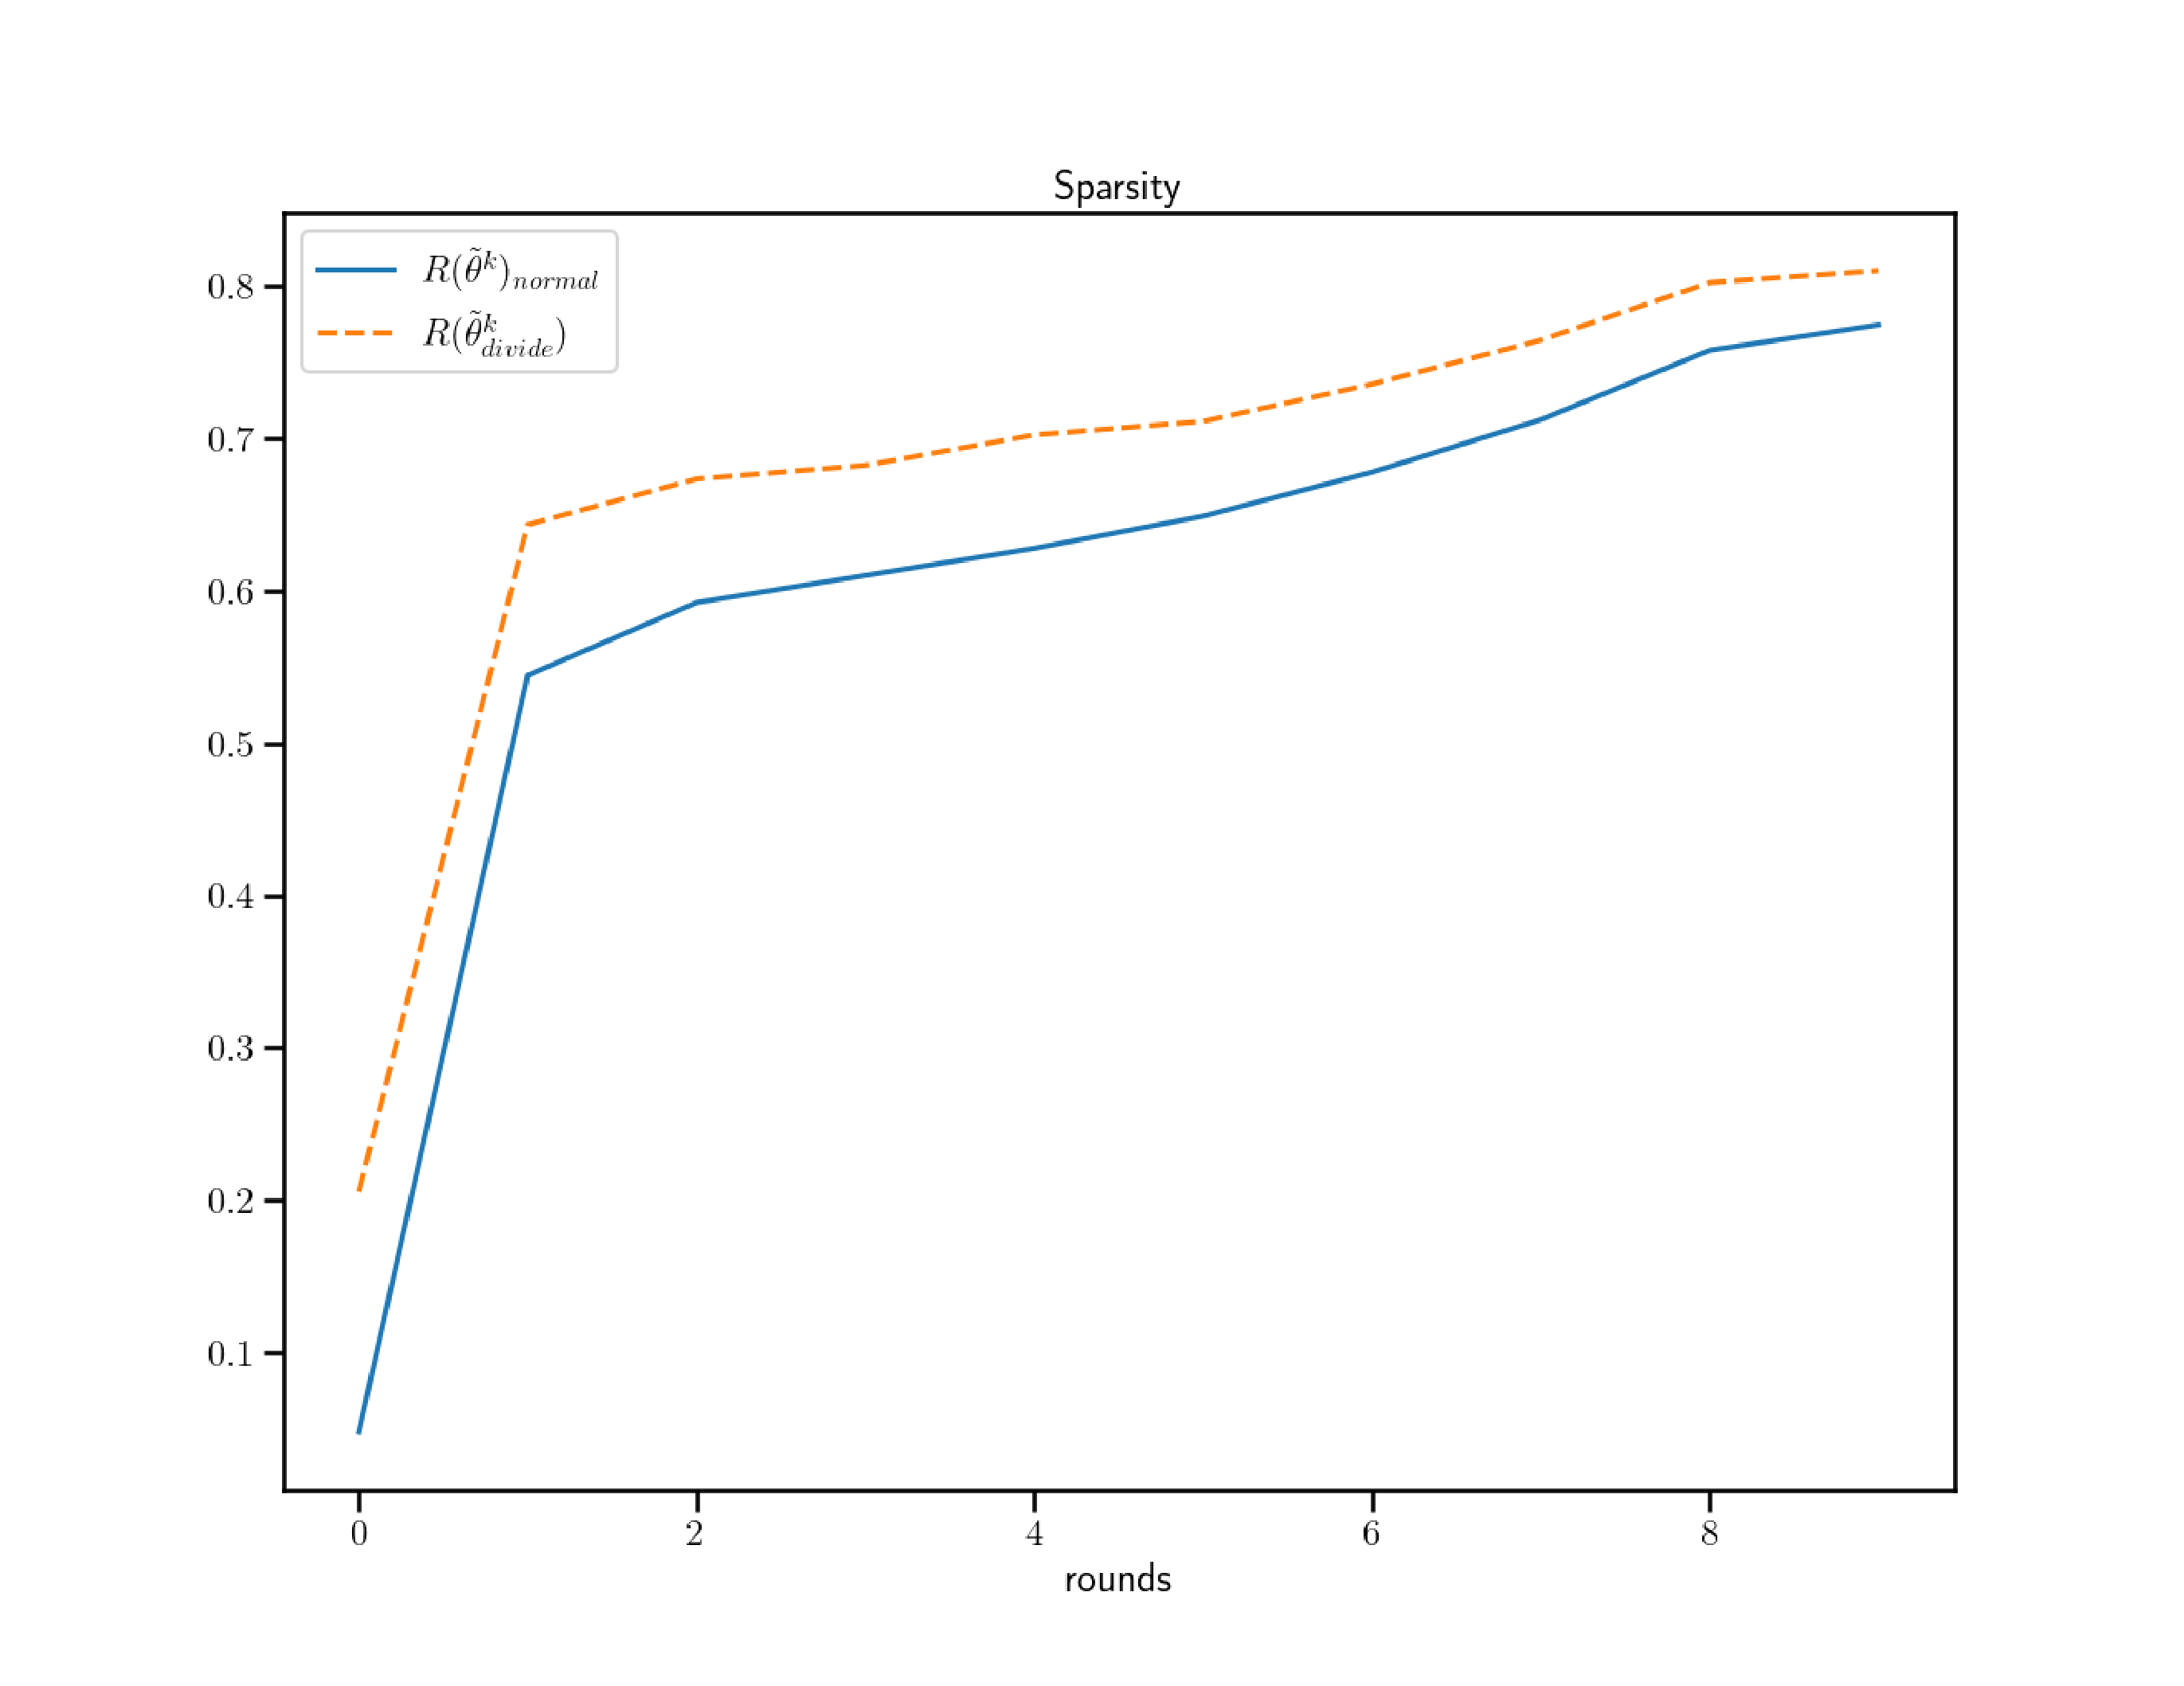
\includegraphics[width = \linewidth]{pic/screening_divide_ratio_long}
	\caption{Screening ratio of dividing method}
	\end{center}	
	\end{figure}

\subsection{Best Divide Method}
We compared the screening ratio with three different methods, including our Divide method, the Dynamic Sasvi method, and a random divide method. 
	\begin{figure}[h]
	\begin{center}	
	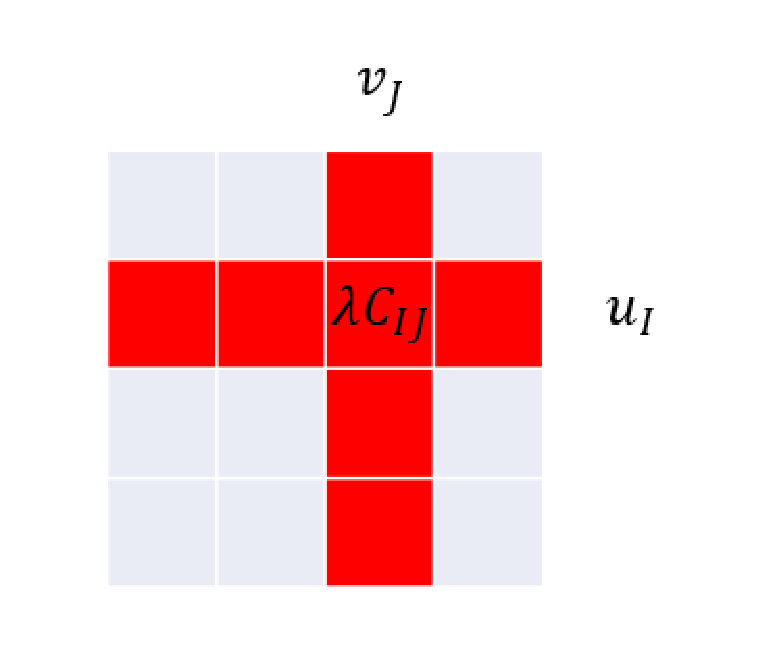
\includegraphics[width = \linewidth]{pic/divide}
	\caption{Comparing of our separation method with random separation method}
	\end{center}	
	\end{figure}

\subsection{Speed up Ratio}

We choose the FISTA method, Newton method, and Language method to test the screening ratio. 
	\begin{figure}[h]
	\begin{center}	
	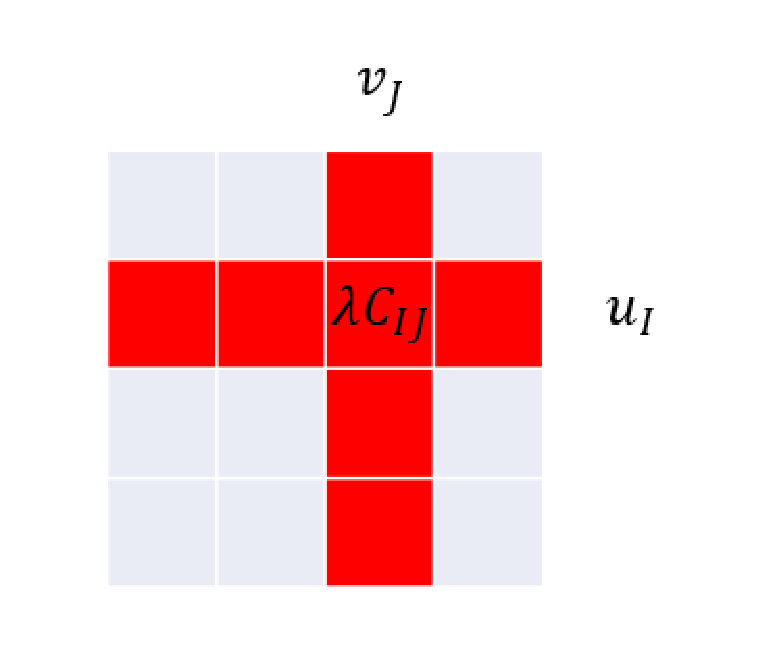
\includegraphics[width = \linewidth]{pic/divide}
	\caption{speed up ratio for different solver}
	\end{center}	
	\end{figure}



\section{CONCLUSION}
Our algorithm is great, we are going to apply the method onto Sinkhorn


\clearpage
\bibliographystyle{apalike}
\bibliography{ref}


%%%%%%%%%%%%%%%%%%%%%%%%%%%%%%%%%%%
%%%%%% SUPPLEMENT (OPTIONAL) %%%%%%
%%%%%%%%%%%%%%%%%%%%%%%%%%%%%%%%%%%

\clearpage
\appendix

\thispagestyle{empty}


% For one-column format, uncomment the following:
\onecolumn \makesupplementtitle
% For two-column format, uncomment the following:
%\twocolumn[ \makesupplementtitle ]

\section{NOTATIONS}
\begin{align}
M &= 
\begin{pmatrix}
\begin{matrix} 1&\\&1 \end{matrix}& & &\dots\dots&\begin{matrix} 1&\\&1 \end{matrix}& & \\
&\ddots& & \ddots\ddots & & \ddots & & \\
& &\begin{matrix} 1&\\&1 \end{matrix}& \dots\dots& & &\begin{matrix} 1&\\&1 \end{matrix}
\end{pmatrix}\\
N &= 
\begin{pmatrix}
\begin{matrix} 1&1&\dots&1&1\end{matrix} &\dots\dots \\
&\ddots\ddots&\\
&\dots\dots & \begin{matrix} 1&1&\dots&1&1\end{matrix}
\end{pmatrix}
\end{align}
\section{PROOFS}
\subsection{Proof of Theorem \ref{Thm:UOT_ShiftProjection}}
For any $p \in {0,1,...,nm -1}$ we assume that $p = (I,J)$, then we can compute that:
 \begin{equation}
\begin{split} 
\vec{x}_p^{\tranT}\tilde{\vec{\theta}} &= \tilde{\vec{u}}_{I} + \tilde{\vec{v}}_J \\
				    &= {\vec{u}}_{I} + {\vec{v}}_J - \max_{0\geq j\geq n} \frac{{\vec{u}}_I +{\vec{v}}_j - \lambda \vec{c}_{p}}{2} - \max_{0 \geq i \geq m} \frac{{\vec{u}}_i +{\vec{v}}_J - \lambda \vec{c}_{p}}{2}\\
				    &= \frac{{\vec{u}}_{I} + {\vec{v}}_J}{2} - \max_{0\geq j\geq n} \frac{{\vec{v}}_j}{2} - \max_{0 \geq i \geq m} \frac{{\vec{u}}_i }{2} + \lambda \vec{c}_{p}\\
				    &= \frac{1}{2}\vec{x}_p^{\tranT}{\vec{\theta}} - \max_{0\geq j\geq n} \frac{{\vec{v}}_j}{2} - \max_{0 \geq i \geq m} \frac{{\vec{u}}_i }{2} +\lambda \vec{c}_{p} \\
				    &\leq \lambda \vec{c}_{p} 
 \end{split} 
\end{equation}
For $\forall p$, we have $\tilde{\vec{\theta}} \in \mathcal{R}^{D}$

\subsection{Proof of Theorem \ref{Thm:AreaScreeningUOT}}
We Generalize the problem as 
\begin{equation}
\max_{\vec{\theta} \in \mathcal{R}^{S}_{I}}{ \vec{\theta}_{I_1} +\vec{\theta}_{I_2} }
\end{equation}
Considering the center of the circle as $\vec{\theta}^o$, we define $\vec{\theta} = \vec{\theta}^{o} + q$, as ${ \vec{\theta}^{o}_{I_1} +\vec{\theta}^{o}_{I_2} }$ is a constant, the problem is equal to $\min_{\vec{\theta} \in \mathcal{R}^{S}_{I}}{- ( \vec{q}_{I_1} +\vec{q}_{I_2} )}$, we compute the Lagrangrian function of later:
\begin{equation}
\min_{\vec{q}} \max_{\eta,\mu,\nu \geq 0} L(\vec{q},\eta,\mu,\nu) =\min_{\vec{q}}\max_{\eta,\mu,\nu\geq0} - {\vec{q}_{I_1} - \vec{q}_{I_2} + \eta( \vec{q}^{\tranT}\vec{q} - r^2)+\mu( a^{\tranT}\vec{q} - e_a ) + \nu( b^{\tranT}\vec{q} - e_b )}
\end{equation}

 \begin{equation}
\begin{split} 
\frac{\partial L}{\partial \vec{q}_i} = \left\{
\begin{aligned}
-1 + 2\eta \vec{q}_i +\mu a_i + \nu b_i \quad& i = I_1, I_2\\
 2\eta \vec{q}_i +\mu a_i + \nu b_i \quad& i \neq I_1, I_2
\end{aligned}
\right.
 \end{split}
\label{eq:lang1}
\end{equation}

 \begin{equation}
\begin{split} 
{\vec{q}_i}^{*} = \left\{
\begin{aligned}
\frac{1- \mu a_i - \nu b_i}{2\eta} \quad& i = I_1, I_2\\
-\frac{\mu a_i + \nu b_i}{2\eta} \quad& i \neq I_1, I_2
\end{aligned}
\right.
 \end{split}
\label{eq:lang1}
\end{equation}

We can get the Lagrangian dual problem:
\begin{equation}
\max_{\eta,\mu,\nu\geq0} L(\eta,\mu,\nu) = \max_{\eta,\mu,\nu\geq0} \frac{\mu a_{I_1} + \nu b_{I_1}-1}{2\eta} +\frac{\mu a_{I_2} + \nu b_{I_2}-1}{2\eta}+ \eta({\vec{q}^{*}}^{\tranT}\vec{q}^{*}-r^2 )+\mu( a^{\tranT}\vec{q}^{*} - e_a ) + \nu( b^{\tranT}\vec{q}^{*} - e_b )
\end{equation}
From the KKT optimum condition, we know that if
\begin{equation}
\begin{split} 
 \eta ({\vec{q}^{*}}^{\tranT}\vec{q}^{*} -r^2) &= 0\\
 \mu( a^{\tranT}\vec{q}^{*} - e_a)&= 0\\
 \nu(b^{\tranT}\vec{q}^{*} - e_b) &=0
 \end{split}
\end{equation}
We set $\eta^{*}, \mu^{*}, \nu^{*}$ as the solution of the equations, which is also the solution of the dual problem. Firstly, we assume that $\eta^{*}, \mu^{*}, \nu^{*} \neq 0$, then the solution is equal to compute the following equations:

\begin{equation}
\begin{split} 
 & (1-\mu a_{I_1}-\nu b_{I_1})^2 + (1-\mu a_{I_2}-\nu b_{I_2})^2 + \sum^{m+n}_{i\neq I_1,I_2}(a_i\mu+b_i\nu)^2 - 4\eta^2 r^2 = 0 \\
 & a_{I_1}-\mu a_{I_1}^2-\nu b_{I_1}a_{I_1} + a_{I_2}-\mu a_{I_2}^2-\nu b_{I_2}a_{I_2} - \sum^{m}_{i\neq I_1,I_2}(a_i^2\mu +b_i a_i\nu) - 2\eta {e_a} = 0 \\
 & b_{I_1}-\nu b_{I_1}^2-\mu b_{I_1}a_{I_1} + b_{I_2}-\nu b_{I_2}^2-\mu b_{I_2}a_{I_2} - \sum^{m}_{i\neq I_1,I_2}(b_i^2\nu +b_i a_i\mu) - 2\eta {e_b} = 0 
 \end{split}
\end{equation}
Rearranged as:
\begin{equation}
\begin{split} 
 & 2-2\mu (a_{I_1}+a_{I_2})-2\nu(b_{I_1}+b_{I_2})+ \|a\|^2\mu^2+\|b\|^2\nu^2+2\mu\nu a^{\tranT}b - 4\eta^2 r^2 = 0 \\
 & (a_{I_1}+ a_{I_1}) - \|a\|^2\mu - a^{\tranT}b\nu - 2\eta {e_a} = 0 \\
 & (b_{I_1}+ b_{I_2}) - \|b\|^2\nu - a^{\tranT}b \mu - 2\eta {e_b} = 0 
 \end{split}
\end{equation}

we have 
\begin{equation}
\begin{split} 
\mu &= \frac{2( e_ba^{\tranT}b - e_a\|b\|^2 )\eta + (a_{I_1}+a_{I_2}) \|b\|^2 - (b_{I_1} + b_{I_2}) (a^{\tranT}b)}{ \|a\|^2 \|b\|^2 -a^{\tranT}b}\\
\nu &=\frac{2( e_aa^{\tranT}b - e_b\|a\|^2 )\eta + (b_{I_1}+b_{I_2}) \|a\|^2 - (a_{I_1} + a_{I_2}) (a^{\tranT}b)}{ \|a\|^2 \|b\|^2 -a^{\tranT}b}\\
 \end{split}
\end{equation}
set it as:
\begin{equation}
\begin{split} 
\mu &= s_1 \eta + s_2\\ 
\nu &= u_1 \eta + u_2
 \end{split}
 \label{eq:final}
\end{equation}

Then we can solve the $\eta$ as a quadratic equation:
\begin{equation}
\begin{split} 
0&=a\eta^2+b\eta+c\\
 a&= 4r^2 - s_1^2\|a\|^2 - u_1^2\|b\|^2 -2s_1 u_1a^{\tranT}b\\
b&=2(a_{I_1} + a_{I_2})s_1 +2(b_{I_1} + b_{I_2})u_1 - 2s_1s_2 \|a\|^2 - 2u_1u_2\|b\|^2 - 2(s_1u_2+s_2u_1)a^{\tranT}b \\
 c&=2(a_{I_1} + a_{I_2})s_2 +2(b_{I_1} + b_{I_2})u_2 -s_2^2\|a\|_1 -u_2^2\|b\|_1 - 2s_2u_2a^{\tranT}b -2
 \end{split}
\end{equation}

Then we can put it back into \ref{eq:final} and get $\mu, \nu$.

If the solution satisfied the constraints $\eta^{*}, \mu^{*}, \nu^{*} > 0$, then it is the solution.
However, if one of the dual variables is less than 0, the problem would degenerate into a simpler question. 

If only $\eta^{*}$ is larger than 0, 
 $\min_{\vec{\theta} \in \mathcal{R}^{S}_{I}}{- ( \vec{q}_{I_1} +\vec{q}_{I_2} )} = -\sqrt{2}r$

If only $\mu^{*}$ or $\nu^{*}$ is less than 0, we are optimizing on a sphere cap, the solution can be found in \cite[Appendix B]{NEURIPS2021_7b5b23f4}

if only $\eta^{*} \leq 0$:
As the sphere is inactivated, the problem gets maximum at every point of the intersection of two planes.
\begin{equation}
\min_{\vec{q}} \max_{\mu,\nu \geq 0} L(\vec{q},\mu,\nu) =\min_{\vec{q}}\max_{\mu,\nu\geq0} - {\vec{q}_{I_1} - \vec{q}_{I_2} +\mu( a^{\tranT}\vec{q} - e_a ) + \nu( b^{\tranT}\vec{q} - e_b )}
\end{equation}
To have a solution, the equations satisfied
 \begin{equation}
\begin{split} 
\frac{\partial L}{\partial q} = \left\{
\begin{aligned}
-1+\mu a_i + \nu b_i =0 \quad& i = I_1, I_2\\
-\mu a_i -\nu b_i \quad =0& i \neq I_1, I_2
\end{aligned}
\right.
 \end{split}
\end{equation}

As the equation satisfied, we can just set $\vec{q}_i^{*} = 0, i \neq I_1,I_2$, then we compute the  
 \begin{equation}
 \min_{\vec{\theta} \in \mathcal{R}^{S}_{I}}{- ( \vec{q}_{I_1} +\vec{q}_{I_2} )} = \frac{a_{I_2}e_b - b_{I_2}e_a -a_{I_1}e_b +b_{I_1}e_a}{a_{I_1}b_{I_2}-a_{I_2}b_{I_1}}
\end{equation}


\end{document}

